%\chapter{統計量を使ったモデルとデータの比較}
\chapter{モデルにおける統計量の性質}
統計モデルからサンプリングを行った標本から、統計量を計算すると、その統計量より偏った値が出現する確率が得られる。この性質を利用して、モデルからサンプリングを行った標本について、統計量がより偏った値が一定値を下回るならば、このモデルからサンプリングされていないと判定を下し、ある特定の値より大きいならば、このモデルから得られた標本であると判断を下す。

%この確率が低いとき、標本がモデルからサンプリングされたものではないと一定の割合で判断を下すことにする。
%このことを利用して、標本をモデルからサンプリングしたと判断するものとそうでないものに仕分けを行う。

%言い換えるなら、ある母数を持つ統計モデルから標本がサンプリングされたのかい?そうじゃないのか?どっちなんだい?に答える方法の一つである。
%これを科学においては、ある母数をもつ統計モデルによって推測してもいいのかい?そうじゃないのかい?どっちなんだい?統計モデルが「ピー」と答える。
%\footnote{本章で説明する仮説検定とは、前者がモデルとの乖離の程度を調べる方法であり、後者は仮説の真偽を調べる数学的方法という点で完全に異なる。}。

\section{自己標本の批判}
統計モデルからサンプリングした標本の統計量が従う確率密度関数が理論的に求められる。
正規モデルの場合、以下の通りである。
\begin{equation*}
    Z = \frac{\sqrt{n}(\bar{x}-\mu)}{\sigma} \sim N(0,1)
\end{equation*}
この性質を利用することで、$Z$値よりも偏った値がどの程度の確率でモデル内で出現するかが計算できる。
例えば、$Z=0$であれば、モデル内でこれ以上に偏った値が出現する確率は約$0.5$程度であり、よくある値または標本であることがわかる。
一方、$Z=1.96$であれば、モデル内でこれ以上に偏った値が得られる確率は約$0.025$程度となり、なかなかレアな値であると思うことができる。
%ここで注意しなければならないのは、$p$値はモデル内における$Z$値よりも偏った値の出現する確率であるということである。
%言い換えれば、現実において$Z$値よりも偏った値の出現する確率についてはなんら言及できていない。
%統計量以上に偏った値がモデルにおいて出現する確率を$p$値という。



\begin{defi}
    統計モデルにおいて、ある統計量よりも偏った(大きいまたは小さな)検定統計量が得られる確率を$p$値と呼ぶ。
    %ある標本から求められた統計量以上に大きな値が得られる確率を$p$値と呼ぶ。
    %絶対にダメと判断されないときは、統計モデルを採択(棄却の対義語)すると宣言しない。
    %統計モデルが棄却されるのは、統計モデルの仮定によって変化する。本書の範囲内であれば、統計モデルの母数、分布関数、独立同一の分布関数からサンプリングされたことによる。
    %最尤統計モデルにおいて、棄却されない統計モデルの母数の範囲を信頼区間といい、棄却されるモデルの母数の範囲を棄却域という。
\end{defi}

モデルでの特定の標本の得られにくさを、$p$値に変換して検討することが可能である。
$p$値が小さいなら、検定統計量$Z$値以上に偏った値の得られる確率が低いということであるので、
$Z$値の元の標本もそもモデルからは得られにくいということを示す。
%つまり、モデルから標本の得られにくさの指標の一つが$p$値であるとも言え、$p$値が小さいほど、その標本はそのモデルから得られにくい。

\if 0
\begin{center}
    標本$\rightarrow$ 統計量 $\rightarrow$ $p$値($p$値の小ささが標本のモデル上での得られにくさの指標になる)
\end{center}
\fi




\subsection{$p$値の計算練習}
%$Z(\bar{x},\mu)$以上の値が得られる確率}
$Z(\bar{x},\mu)\sim N(0,1)$により、$Z$以上の値が得られる確率の計算を練習してみよう。つまり、以下をコンピュータに計算させる。
\begin{equation*}
    p = \varPhi(Z(\bar{x},\mu)>x)
\end{equation*}
正規モデル$M(\mu=168;\sigma^2=6.8)$から得た標本の統計量を、$\bar{x}=172.4$、サンプルサイズを$n=10$とした。
$Z$値は$Z(\bar{x},\mu)=2.04$となる。これを元に、以下のスクリプトを実行すると、$p$値が約$0.04$程度であることがわかる。

\begin{lstlisting}
xbar = 172.4
mu = 168
sigma2 = 6.8**2
n=10
Z = np.sqrt(n)*(xbar-mu)/np.sqrt(sigma2)
print(Z)
p=1-norm.cdf(Z,0,1)
print(p*2)
\end{lstlisting}



\subsection{自己標本の否定確率}
%ここから、いくつか数学的な構造について紹介する。
%この内容は科学において使うのは非常に難しい。
%例えば、有意水準$\alpha$や検定量$\beta$などを決定することはできない。
%$Z_i$がモデル由来であるかを自己標本の批判を元に判断する。

正規モデル$M$において、$M$の標本を得てその検定統計量Zが極端な値を取るとき、$M$の標本ではないと判定する。
ここで、極端な値とは、$Z$が標準正規分布に従うことから、標準偏差の2よりも偏った値である場合に、$M$の標本ではないとする。
このとき、標準正規分布表を参照すれば$P(|Z|>2)=0.02275\times 2=0.046$程度となる。

標準偏差の代わりに確率を元に判定を行う。
$P(|Z|>2)=0.046$はキリが悪いので代わりに、$P(|Z|>x)=0.05$を設定する。
標準正規分布表を参照すれば$P(|Z|>x)=0.05$となるのは$x=1.96$程度である。
この値よりも大きな$|Z|$となる標本は、$M$の標本ではないと判定する。

あるモデルの検定統計量がより偏った値を取る確率$0.05$を他の統計モデルでも適用すれば、さまざまなモデルで統一的に判定が行える。また、あるサンプルサイズの標本を100個モデルからサンプリングした場合、$95$回はモデルから生成されたものと判断し、残りの5回についてはモデルから生成されていないと判断する。


\begin{defi}
 モデルからサンプリングされた標本のうち、偏っていると判定する割合を$\alpha$とし、有意水準と呼ぶ。
 %$言い換えれば、$\alpha$値は、統計モデルからサンプリングされた値について、これが元の統計モデルからサンプリングであることを判定する閾値\footnote{閾値(読み:いきち)=限界値}である。
\end{defi}

%本書では、上記の歴史的な事情にしたがって、$\alpha=0.05$を利用して、理論計算を行う。

%これは、モデル$M$の標本であるはずなのに、外れた値であれば、そのモデル$M$
%モデルが生成したはずの標本であるが、閾値を決めてモデルから生成されたものではないとするのである。
%モデルが自身から得られた標本を批判するのであるから、自己の標本を批判するのである。
%これは、モデルを元に、標本がモデルにより予測できるかどうかを考えている。


%具体的には、正規モデルを利用すれば、その統計量$Z$が$N(0,1)$に従うことがわかっている。
%$Z$の値が偏った値になっていれば、その出現頻度は低くなるので、$P(|z|<Z)=95/100$となる$Z$を計算する。
%この$Z$は具体的に計算でき、$Z_{0.95}=1.96$である。
%ここから、$|z_i|<Z_{0.95}=1.96$となる$z_i$の個数を数えればおよそ$95$になる。
%また、$|P(|z_i|>0.95)| > 1.96$ならば、$|z_i|>Z_{0.95}=1.96$である。


%統計モデルの分布関数が変化すれば、その統計モデルにおける信頼区間・棄却域の値も変わる\footnote{中心極限定理を利用し、統計量の出現範囲を近似することが多い。}。
%実際のデータが$\alpha\%$の割合で棄却されるということではない。モデルから生成された標本であるのに、この統計モデルから生成されていないと疑いをかける。

\subsection{母数平均の変化に応じた信頼区間}
%$95\%$信頼区間と$p$値の関係}
正規モデル$M$においてその検定統計量$Z$について、式変形を行う。
\begin{eqnarray}
    & &|Z| < z_{0.025}( = 1.96 ) \notag \\
    &\rightarrow& \frac{\sqrt{n}|\bar{x}-\mu|}{\sigma} < z_{0.025} \notag\\
    &\rightarrow& \mu-\frac{\sigma}{\sqrt{n}}z_{0.025} < \bar{x} < \mu+\frac{\sigma}{\sqrt{n}}z_{0.025} \label{confidence_interval_eqn}
\end{eqnarray}

\begin{defi}
式\eqref{confidence_interval_eqn}の$\bar{x}$の区間を信頼区間といい、次の式で定義される。
\begin{equation*}
    A=\{x;\mu-\frac{\sigma}{\sqrt{n}}z_{0.025} < x < \mu+\frac{\sigma}{\sqrt{n}}z_{0.025} \}
\end{equation*}
これ以外の区間を棄却域と言う。ここでは、$R=\mathbb{R}\backslash A$が棄却域である。
% Comment
%信頼区間の定義は、検定統計量の範囲ではなく、平均値の範囲
\end{defi}
信頼区間の範囲は、サンプルサイズ$n$、有意水準$\alpha$およびモデルの母数$\mu,\sigma^2$により決まる。

まず、$\mu$の変化に応じて、信頼区間が変化する様子を確かめる。
図\ref{fig:confidence_interval_model}には、モデル毎の平均値と信頼区間を描いた。$\mu$の大きさにによらず信頼区間の幅は同じである。
各$\mu$に対して、信頼区間の内側で$\bar{x}$が$95\%$の確率で見つかることを統計モデル$M(\mu)$が推測する。
この外側にある$\bar{x}$になる標本については、偏っていると判定する。
%統計モデルの標本ではないと判定を下す。

\begin{figure}
    \begin{center}
        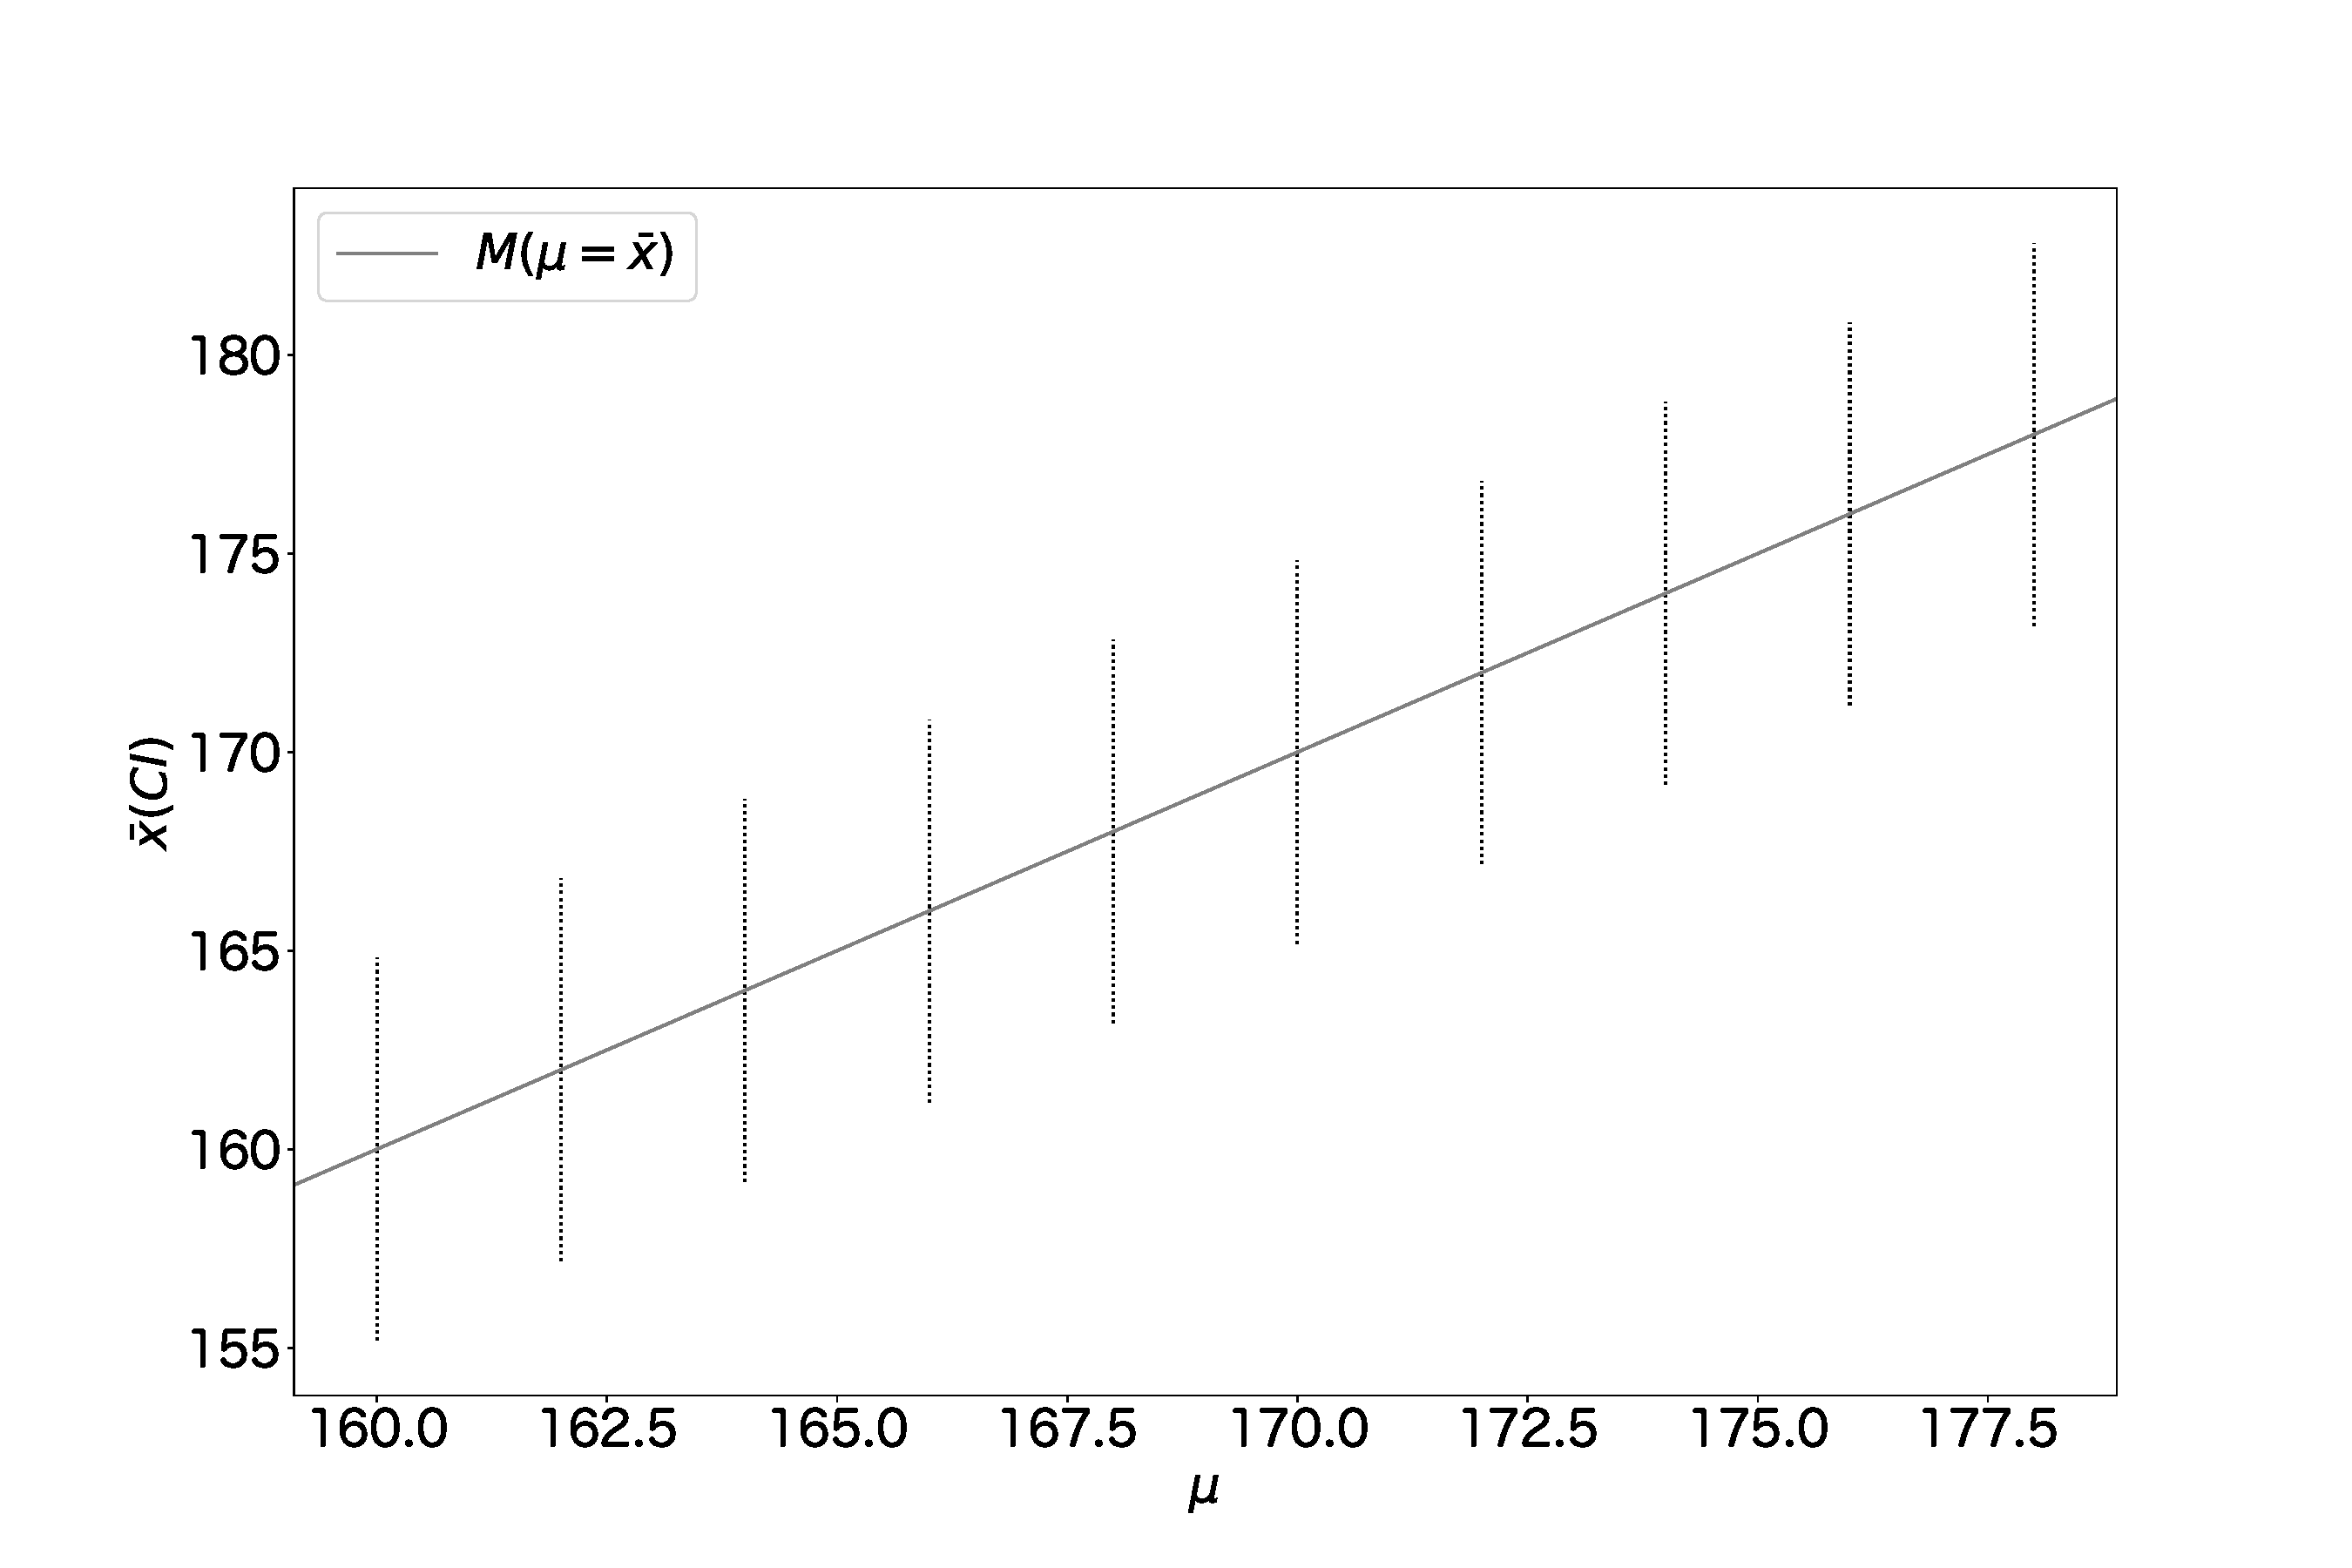
\includegraphics[width=10cm]{./image/04_/confidence_interval_model.pdf}
        \caption{横軸にモデルの母数$\mu$、縦軸に、モデルが予測する平均値$\bar{x}$、エラーバーに$95\%$信頼区間を描いた。$N=10,\sigma^2=6.8^2$}
        \label{fig:confidence_interval_model}

    \end{center}
\end{figure}



\section{統計量をもとにしたモデル間類似度(検出力)}
母数の異なる二つの統計モデル$M_a,M_b$について考察する。
$M_a$の信頼区間内の検定統計量が$M_b$において出現する確率を検出力という。
%言い換えれば一方で出現する統計量が他方のモデルにおいて出現する確率である。
これは、$M_a$から$M_b$への統計量を元にしたモデル間類似度と言える。

\subsection{検出力の定義}
$M_a$におけるある統計量についてその信頼区間を$A_a$とするとき、$A_a$が$M_b$において出現する確率を$\beta$とする。
具体的には以下の式で表される。
\begin{eqnarray*}
    & &P_a(\vecc{X} \in R_a) = \alpha\\
    & & P_b(\vecc{X} \in A_a) = P_b(\vecc{X} \notin R_a )=\beta
\end{eqnarray*}
ここで、$R_a,A_a$はそれぞれ統計モデル$M_a$の棄却域、信頼区間を表し、$P_a,P_b$は、それぞれ統計モデル$M_a,M_b$におけるある統計量がしたがう分布の密度関数。
$1-\beta$を検出力という\footnote{検出力を検定力または統計力と呼ぶこともある。\\ \url{https://id.fnshr.info/2014/12/17/stats-done-wrong-03/}}。


検出力$1-\beta$は、二つの異なるモデルを検定統計量を基準に比較するための指標である。
%$1-\beta$が$1$に近ければ、
二つの統計モデルの母数がよく一致するならば、$1-\beta$は$\alpha$に近い値を取り、また母数が一致している$M_a$に対する$M_a$の検出力は、$\alpha$である。
一方、モデルの母数が一致していないならば、$1-\beta$は$1$に近い値を取る。
%$M_a$を棄却する閾値を低く設定すると、$\beta$は大きな値になる。

$\beta$は$\alpha$を変数にする関数になっており、
$\alpha$を0に近づけていくと、信頼区間は徐々に大きくなり、検出力$1-\beta$は小さくなる。
$\alpha$を大きくすると、信頼区間は徐々に狭くなり、検出力$1-\beta$は大きくなる。



\subsection{正規分布モデルの検出力}
正規モデルをつかって、$P_a(\vecc{X} \in R_a),P_b(\vecc{X} \in A_a)$を計算する。
$\sigma^2$がすでに与えられた正規モデルを$M(\mu;\sigma^2)$とし、$M_a=M(\mu_a),M_b=M(\mu_b)$とする。
$M_a$または、$M_b$における実現値の平均値$x_a,x_b$は、それぞれ$N(\mu_a,\sigma^2/n), N(\mu_b,\sigma^2/n)$に従う。
また、$M_a$の信頼区間$A_a=\{\vecc{x}; |\bar{x}| <\mu_a+\sigma / \sqrt{n}z_{2.5\%} \}$である。
このとき、$P_a$を$N(\mu_a,\sigma^2/n)$の確率密度関数とすると、
\begin{equation*}
    P_a(\vecc{X} \in A_a) = 1-\alpha
\end{equation*}
であるのは定義から明らか。
また、$P_b$を$N(\mu_b,\sigma^2/n)$の確率密度関数とすると、
\begin{equation*}
    P_b(\vecc{X} \in A_a ) = \beta
\end{equation*}
である。

\begin{figure}
\begin{center}
 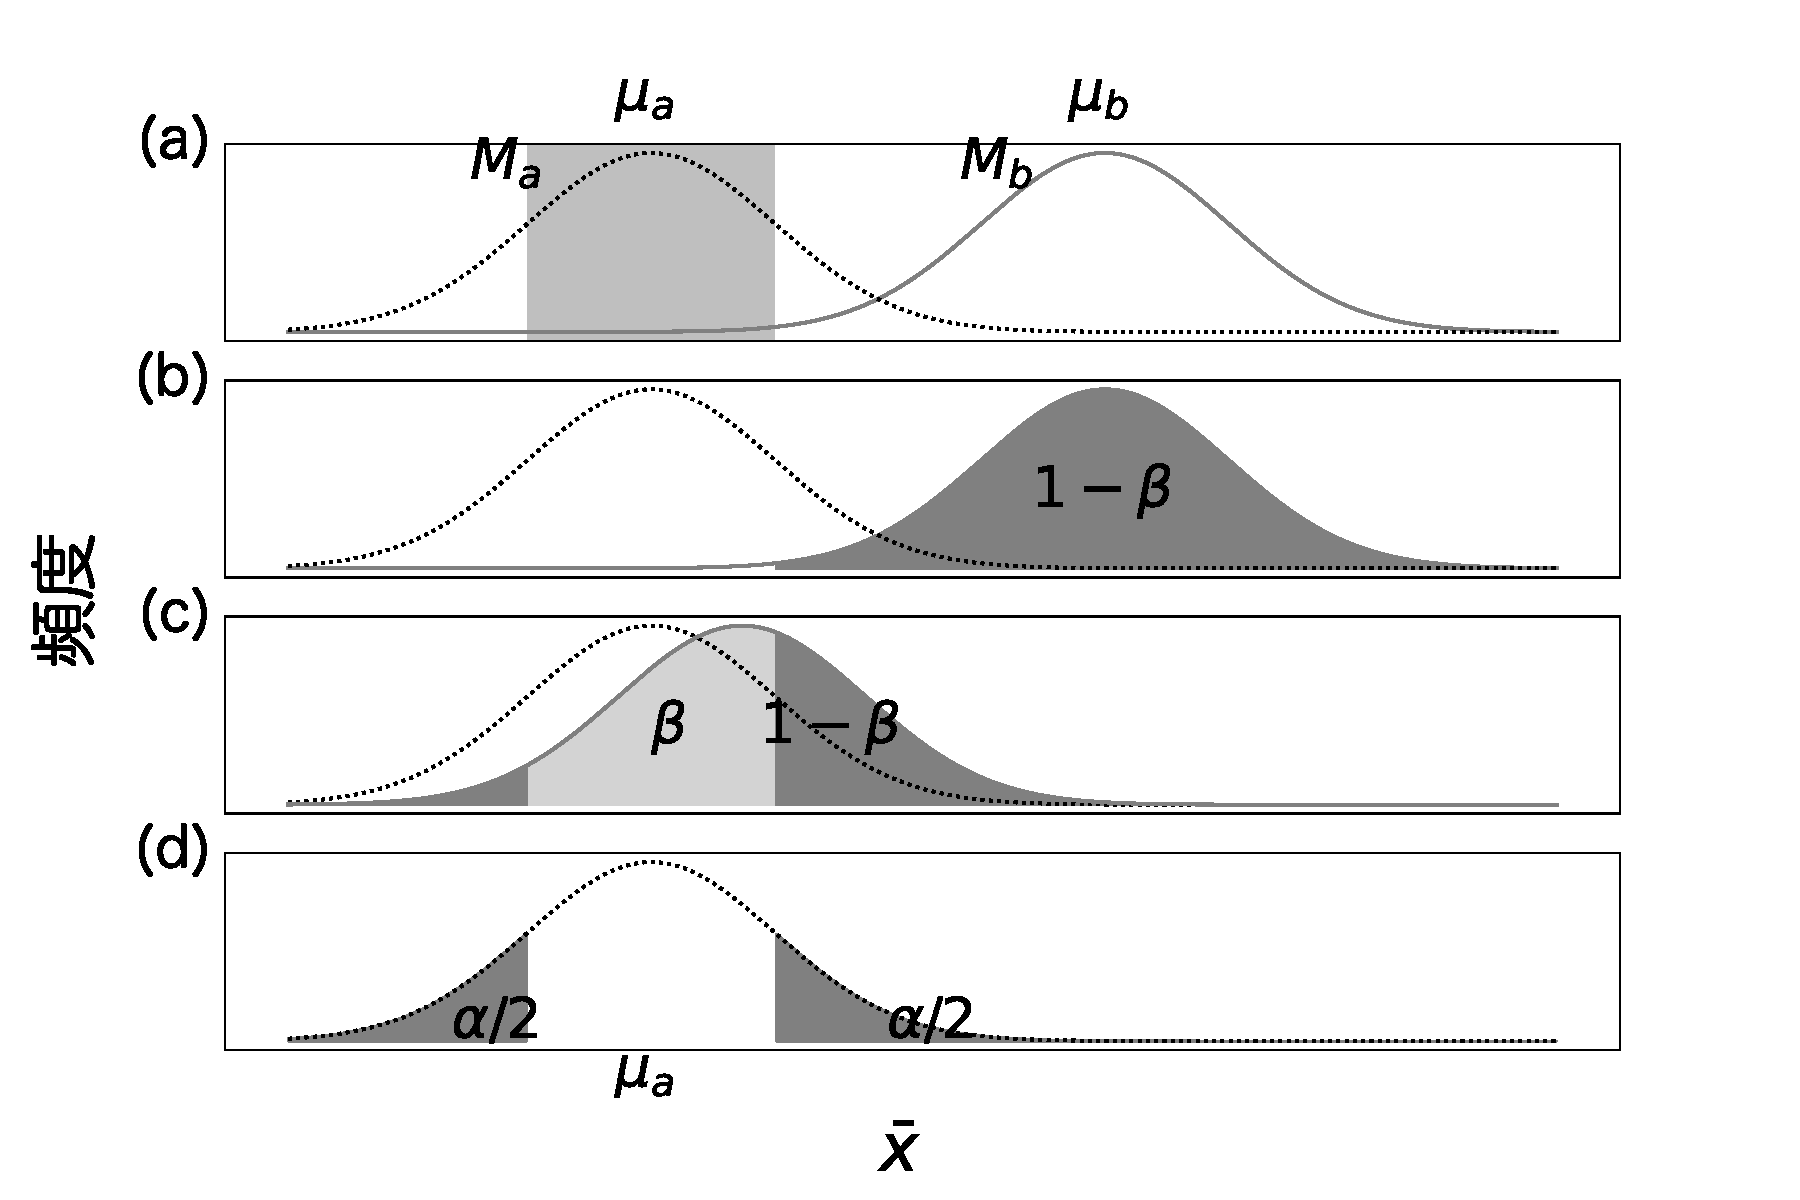
\includegraphics[width=15cm]{./image/04_/power_of_a_test_2.pdf}
 \caption{統計モデル$M_a,M_b$から計算された統計量$\bar{x}$の確率分布$P_a,P_b$。(a)灰色の範囲は$M_a$の信頼区間。(b)灰色の領域は、$1-\beta$の領域を示している。$\beta$の面積が非常に小さいので、グラフ上に描画できていない。(c)$\mu_b$が$\mu_a$に近いときの$\beta$と$1-\beta$の領域。(d)灰色の範囲の面積が$\alpha$を示している。}
 \label{fig:power_of_test_alpha_beta}
\end{center}
\end{figure}


図\ref{fig:power_of_test_alpha_beta}に検出力と$\alpha$の領域を図示した。
%$M_a$の$95\%$信頼区間は、$|\mu|<\mu_a+z_{0.025}\frac{\sigma}{\sqrt{N}}$とした。
信頼区間は、図\ref{fig:power_of_test_alpha_beta}(a)において灰色で塗った$x$軸の範囲である。$\alpha$は図\ref{fig:power_of_test_alpha_beta}(d)の灰色で塗りつぶした領域の面積である。
検出力$1-\beta$は、$M_b$における$M_a$の信頼区間の外側の領域の面積なので、図\ref{fig:power_of_test_alpha_beta}(b)の濃い灰色の範囲である。
図\label{fig:power_of_test_alpha_beta}(c)は、$M_b$の母数$\mu_b$を$M_a$の母数$\mu_a$に近付けたときの$\beta,1-\beta$。



\begin{figure}
    \begin{center}
        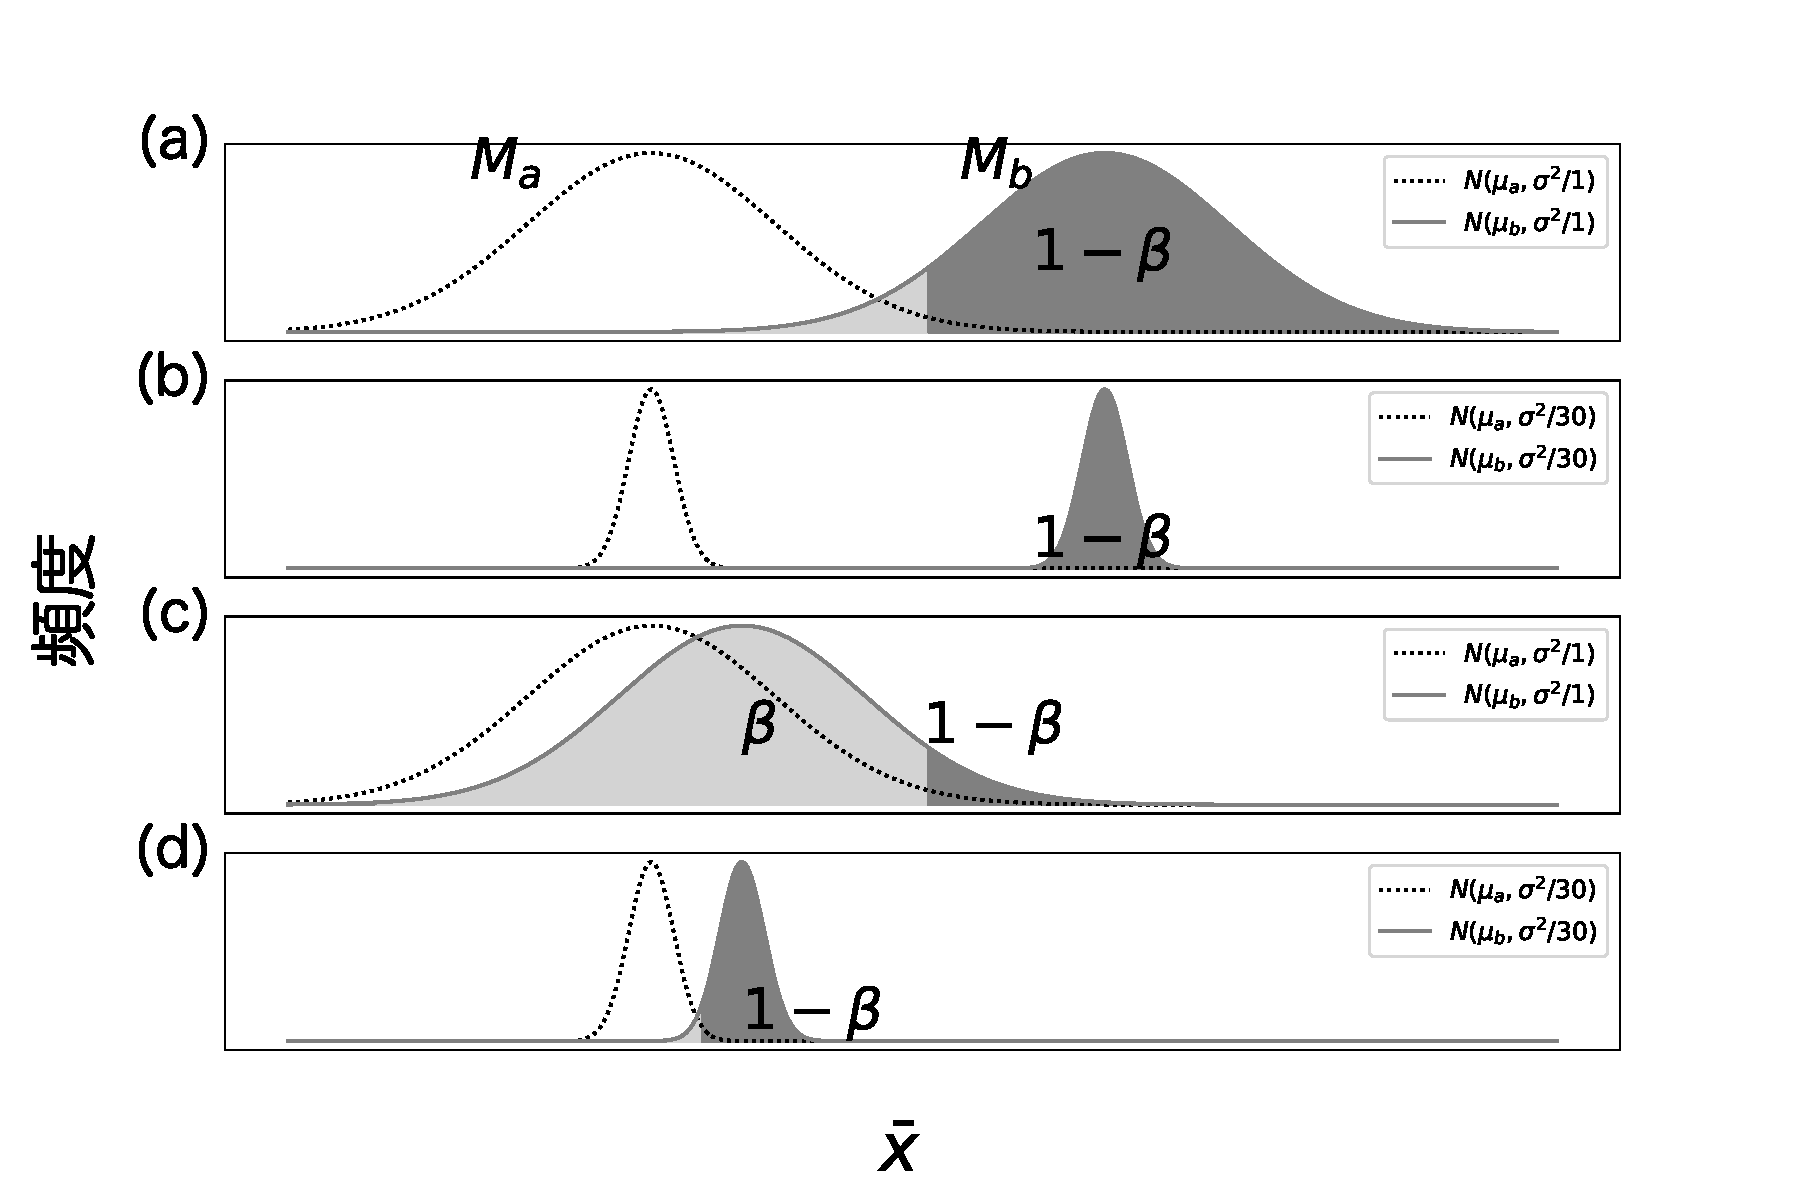
\includegraphics[width=15cm]{./image/04_/power_of_a_test_3.pdf}
        \caption{統計モデル$M_a,M_b$から計算された統計量$\bar{x}$の確率分布$P_a,P_b$。(a)$\mu_a,\mu_b$のサンプルサイズ$1$の平均値がしたがう確率密度関数$N(\mu_a,\sigma^2/1),N(\mu_a,\sigma^2/1)$。(b)(a)と同じ$\mu_a,\mu_b$に対して、サンプルサイズを$30$にした場合の確率密度関数。(c)$\mu_a,\mu_b$が(a)よりも近いときの$\bar{x}$の確率密度関数。(d)(c)と同じ$\mu_a,\mu_b$に対してサンプルサイズを$30$にした場合の$\bar{x}$の確率密度関数。}
        \label{fig:power_of_test_alpha_beta_sample_size}
    \end{center}
    \end{figure}

\paragraph{サンプルサイズによる$\beta$の変化}

$\alpha$、$M_a$の母数平均$\mu_a$、$M_b$の母数平均$\mu_b$を固定したまま、サンプルサイズを変化させ,
$\beta$の変化を図\ref{fig:power_of_test_alpha_beta_sample_size}に示す。$\bar{x}$が従う分布($N(\mu,\sigma^2/n)$)の分散がサンプルサイズによって変化することは明らかである。このことから、サンプルサイズが大きくなると、信頼区間は徐々に狭くなり、$1-\beta$は大きくなる。サンプルサイズが小をさくすると$1-\beta$も小さくなる。

\paragraph{モデルの母数による$\beta$の変化}
$\mu_a$を固定し、$\mu_b$を変化させたときの検出力$1-\beta$を図\ref{fig:power_of_test_N_mu0_variable}に示した。
%モデルの母数平均$\mu_a,\mu_b$と$\beta$の関係について考察する。
$\mu_a$と、$\mu_b$が一致していれば、$P_b(\vecc{X} \in A_a )$は$1-\alpha$になる。
$\mu_b$が$\mu_a$から離れていくと、$P_b(\vecc{X} \in A_a)=0$に近づいていく。

\paragraph{$\alpha$による$\beta$の変化}
$\alpha$が小くなれば、信頼区間の幅が大きくなり、$1-\beta$も小くなる。
$\alpha$が大きくなれば、信頼区間の幅が小くなり、$1-\beta$も大きくなる。

%ここまでをまとめると、検出力は、モデルの母数、サンプルサイズ、有意水準によって変化する。


\begin{figure}
    \begin{center}
        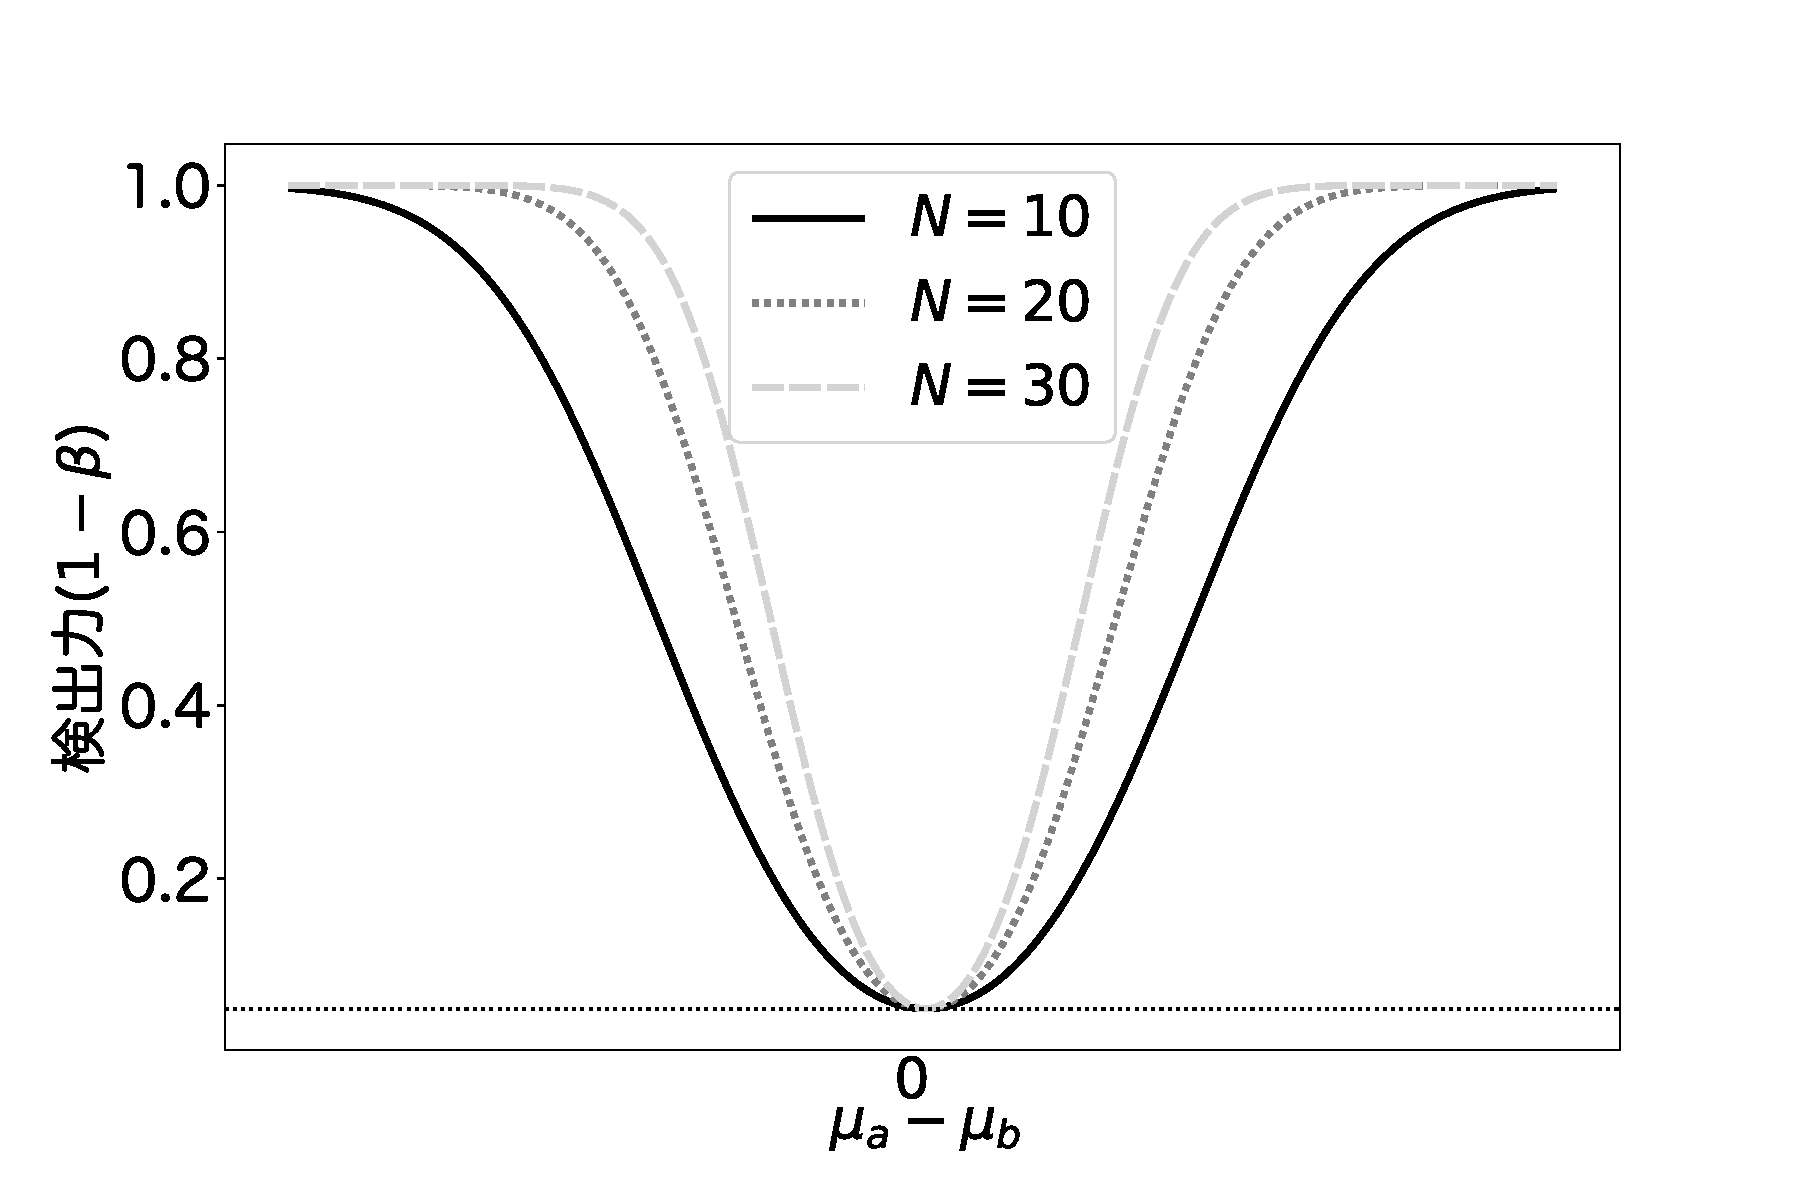
\includegraphics[width=15cm]{./image/04_/power_of_test.pdf}
        \label{fig:power_of_test_N_mu0_variable}
        \caption{$\mu_a$を変数にしたときの検出力(検出力関数)。}
    \end{center}
\end{figure}

\subsection{$\beta$の計算}
正規モデル$M_a,M_b$を使って、$\beta$を計算する。
$M_a$の信頼区間は、
\begin{equation*}
    -z_{0.025}\leq \frac{\sqrt{n}(\bar{x}-\mu_a)}{\sigma}\leq z_{0.025}
\end{equation*}
より、
\begin{equation*}
    A_a = \{ \vecc{x} ; \mu_a -\frac{\sigma}{\sqrt{n}}z_{0.025} \leq \bar{x} \leq \mu_a +\frac{\sigma}{\sqrt{n}}z_{0.025} \}
\end{equation*}
である。ここで、$a=\mu_a -\frac{\sigma}{\sqrt{n}}z_{0.025},b = \mu_a +\frac{\sigma}{\sqrt{n}}z_{0.025} $とおく。棄却域は$A_a$以外の要素である。$M_b$の標本平均$\bar{x}_b$は、$N(\mu_b,\frac{\sigma^2}{n})$に従うので、その確率密度関数において、$A_a$が出現する確率が$\beta$である。
%ここで、$\frac{\sqrt{n}(\bar{x}_b-\mu_b)}{\sigma}\sim N(0,1)$である。
このことを利用すると、
$a,b$は、$N(\mu_b,\frac{\sigma^2}{n})$の実現値だとすると、$a,b$を標準正規分布へ規格化したときの実現値をそれぞれ$a',b'$とする。
すると、$a'$は以下の計算式により求められる。
\begin{eqnarray*}
 a' &=& \frac{\sqrt{n}(a-\mu_b)}{\sigma} \\
    %&=& \frac{\sqrt{n}(\mu_a-\frac{\sigma}{\sqrt{n} z_{\alpha/2}})}{\sigma}\\
    &=& -z_{\alpha/2}+\frac{\sqrt{n}}{\sigma}(\mu_a-\mu_b)
\end{eqnarray*}
同様に、$b'$は以下の通り。
\begin{eqnarray*}
 b' &=& \frac{\sqrt{n}(b-\mu_b)}{\sigma} \\
    %&=& \frac{\sqrt{n}(\mu_a-\frac{\sigma}{\sqrt{n} z_{\alpha/2}})}{\sigma}\\
    &=& z_{\alpha/2}+\frac{\sqrt{n}}{\sigma}(\mu_a-\mu_b)
\end{eqnarray*}
以上より、$-z_{\alpha/2}+\frac{\sqrt{n}}{\sigma}(\mu_a-\mu_b) \leq x\leq  z_{\alpha/2}+\frac{\sqrt{n}}{\sigma}(\mu_a-\mu_b)$の間での$N(0,1)$の確率密度関数の積分値が$\beta$である。


\paragraph{計算}

$d=\frac{\mu_a-\mu_b}{\sigma}$とおく。$d=0.6,n=9$とする。このときの$\beta$を計算する。
$N(0,1)$において、$-z_{\alpha/2} -0.6\sqrt{n} \leq x \leq z_{\alpha/2} +0.6\sqrt{n}$の区間で積分する。

\begin{lstlisting}
A,B = norm.interval(0.95,0.,1)
N = 9
d = 0.6
a,b = A+d*np.sqrt(N),B+d*np.sqrt(N)
print(a,b)
norm.cdf(b,0,1)-norm.cdf(a,0,1)
\end{lstlisting}

答えは、$0.564$
\begin{comment}
\subsection{最尤モデルでの$\beta$の計算}
\subsubsection{データを元にしたモデルとモデルの類似度}
統計モデルAを$M(\mu=170)$とし、統計モデルBを$M(\mu=168)$とする。
標本の大きさを$100$とすると、モデルA,Bの間の検出力が以下のプログラムにより計算できる。
%$d=\frac{170-\bar{X}}{6.8}$、$n=100$であるので、$\bar{X}=168$を得たとすると、
\begin{lstlisting}
A,B = norm.interval(0.95,0,1)
N = 100
d = (170-168)/(6.8)
a,b = A+d*np.sqrt(N),B+d*np.sqrt(N)
print(a,b)
norm.cdf(b,0,1)-norm.cdf(a,0,1)
\end{lstlisting}
検出力は、$0.163$
\end{comment}


\section{過誤のまとめ}
これまでの議論をまとめる。モデル$M_a$の標本について、モデル$M_a$に関する標本であるかを判定する。標本の検定統計量のうち頻度$\alpha$程度を$M_a$の標本ではあにと判断する。このように、モデル$M_a$から生成されたのに、モデル$M_a$から生成したものではないと言う誤った判断を行う事になる。この判断の間違いを第1'の過誤と呼ぶ。

次に、モデル$M_b$から得られた標本が、別のモデル$M_a$の標本かどうかを判定することを考える。この場合、検定統計量が$M_a$の信頼区間含まれているかどうかを確認し、含まれていない場合には、モデル$M_a$からサンプリングされた標本ではないと判定する。検定統計量が信頼区間に含まれている場合、実際には$M_a$の標本ではないにもかかわらず、誤って$M_a$の標本であると判断することになる。この誤った判断を第2'の過誤と呼ぶ。以上のことをまとめると、表\ref{table:type_error}のようになる。

\begin{table}[hbtp]
 \caption{モデル$M_a$による自己標本批判}
 \label{table:type_error}
 \centering
 \begin{tabular}{ccc}
  \hline \hline
  &  $M_a$の信頼区間に &  $M_a$の信頼区間に \\
  & 標本の統計量が入っていない & 標本の統計量が入っている \\
  \hline 
  モデル$M_a$の標本  & モデル$M_a$の標本ではないと判定  & モデル$M_a$の標本と判定 \\
  & (第1'の過誤) & \\
  %  & $\alpha$ &  $1-\alpha$\\
  モデル$M_b$の標本  & モデル$M_a$の標本ではないと判定  & モデル$M_a$の標本であると判断 \\
  & & (第2'の過誤) \\
  %& $1-\beta$ & $\beta$ \\
  \hline
 \end{tabular}
\end{table}


\begin{SMbox}{正解と回答の違い}
 あるデータ群に対してそのデータの特徴を元に、YesまたはNoとアノテーションをつける。
 データからそのYesまたはNoを予測する手順を開発する。
 その手順によって得た回答と、正解(真の値)の一致と不一致は以下の通りになる(表\ref{table:Yes_no_answer})。
 回答と一致したら、True、一致しないならFalse。
 Yesと予測したらPositive、Noと予測したらNegativeとする。
 回答がYesな問題に、Yesと答えることは(手順が正しい予測を行なった)、True Positiveといい、Noと答える(手順が間違えた予測を行なった)ことはFalse Negativeという。回答がNoな問題に、Yesと答えることを、False Positive、また、Noと答えることをTrue Negativeという。

統計モデル$M_a$により、標本を$M_a$のものと$M_b$のものに分ける作業をおこなう。 具体的には、モデル$M_a$の標本にYesを対応ずけ、モデル$M_b$の標本にNoを対応付ける。標本を元に、YesまたはNoを判定する手順をモデル$M_a$において信頼区間に統計量が入っているかいなかをもとに判断する。この問題において回答がFPとなったものが第1'の過誤であり、FNとなったものが第2'の過誤である。
\end{SMbox}

\begin{table}[hbtp]
 \caption{正解と回答の違い}
 \label{table:Yes_no_answer}
 \centering
 \begin{tabular}{ccc}
  \hline \hline
  &  負例(真の値) & 正例(真の値)  \\
  \hline 
  正例(予測値) &  偽陽性(FP)  & 真陽性(TP)\\
  &予測が外れた & 予測が当たった\\
  負例(予測値) & 真陰性(TN) & 偽陰性(FN)\\
  & 予測が当たった & 予測が外れた\\
  \hline
 \end{tabular}
\end{table}

\subsection{サンプルサイズの設定}
統計モデル$M_a$により、標本を$M_a$のものと$M_b$のものに分ける作業をおこなう。
このとき、なるべくなら第2'の過誤を少くしたい。
これは、$1-\beta$をなるべく大きく設定ことで解決できる。
ここで、モデルの母数は固定であり、有意水準についても$\alpha$と決定しているものとする。
サンプルサイズを適切な値に設定することで、$1-\beta$を特定の値にできる。
そこで、サンプルサイズの具体的な計算を行う。

%$\beta$の数値、モデルの母数、有意水準を固定したとき、必要なサンプルサイズを計算することができる。%ここでは、$\mu_a,\mu_b$が固定されている状況を考える。
%検出力$1-\beta$は$1$に近いほど、
%検定統計量を基準にして$M_a,M_b$の違いを。
%あらかじめ決めたおいた基準の$1-\beta$を設定し、それ以上の$1-\beta$となるサンプルサイズを推測する。
%サンプルサイズが小さければ、$M_a$と$M_b$の違いは検定統計量を基準にして曖昧であり、サンプルサイズが大きくなると、統計量の出現頻度の違いが明らかになる。
\subsubsection{サンプルサイズ}
$M_a$と$M_b$の母数平均の差$d$と検出力を指定したときに、$M_a,M_b$間の検出力をある値以上にするための最小のサンプルサイズが計算できる。
$\beta=0.1,d=0.8$とし、この$\beta$を満たすように$N$を計算した。

\begin{lstlisting}
A,B = norm.interval(0.95,0.,1)
beta = 0.1
d = 0.8
for N in range(10,200,2):
    a,b = A+d*np.sqrt(N),B+d*np.sqrt(N)
    beta_ = norm.cdf(b,0,1)-norm.cdf(a,0,1)
    if beta_ < beta:
        break
print(N)
\end{lstlisting}
二つのモデルの間の検出力を$0.9$以上にするために必要な最小のサンプルサイズは、$18$であることがわかる\footnote{正規モデルでは}。

\section{自己否定の誤推定}
統計モデルからサンプリングされた標本を、統計量により元のモデルからサンプリングされたかどうかを判断するとき、ある特定の処理を途中に加えることで、そのモデルからサンプリングされた標本ではないと想定以上に判断してしまうことがある。言い替えると、複数の標本のうち$\alpha$程度の標本をモデルのものではないと判断したいにもかかわらず、適切な処理や計算を行わないことで、$\alpha$より多くの標本にこのモデルの標本ではないと判断をくだすことになる。
そのような処理や計算方法について説明をおこなう。
\begin{defi}
  $p$値の分布が偏ることで、$p<\alpha$となる確率が$\alpha$ではないことを「有意水準$\alpha$で検定ができないと言う」。
\end{defi}


%このような過度な推定は、二つの要素に分解できる。
%不適切な統計量を使用することで、棄却域と統計量の違いにより生じる$\alpha_1$、そして、様々な種類の途中処理を噛ませて計算した結果生じる$\alpha_2$である($0<\alpha_2 \leq 1$)。

%$\alpha_2$は、$\alpha\times 2$以上になる場合、軽視されることはないが、
%$\alpha_1$が同程度の隔たりになる場合においては無視され、$\alpha_1$は$\alpha_2$よりも軽視されがちである。
%この過誤は2つの要因に分解でき、\footnote{$\alpha_2$は$\alpha_1$に関係するので実際には、分解できない。気持ちとしては、$\alpha_2$は、$\alpha_1$を変数に持つ関数である$\alpha=\alpha_2(\alpha_1)$。}、
%$\alpha_2=\alpha$となっていれば、有意水準$\alpha$の検定ができる。

%統計モデルに対して不適切な統計量を使ってモデルの検証を試みると、第一の過誤が変化することがわかっている。
\subsection{有意水準$\alpha$で検定が行えている}
$X\sim N(\mu,\sigma^2)$について、これを、累積分布関数により、$x$以下の数値が出現する確率に変換する。$F$を確率密度関数とすると、$F(X<x)$を計算する。
これは、$0\sim 1$の間で一様に分布する。このことを確かめる。

正規分布から$10^5$回サンプリングを行い、その累積分布関数により、サンプリングした数値より小さな値が出現する確率を計算した。
結果は、\ref{fig:test_cummlative_distribution}の通り$F(X<x)$が、傾き$1$の直線上に乗る\footnote{一様分布している}。

この性質を使うことで、有意水準$\alpha$で検定が行えていることを数値計算により確かめることができる。
具体的には、検定統計量を計算し、これが従う分布形の累積分布関数により統計量より小さな値が出現する確率を計算する。これを複数の標本について行うと、計算された値が一様分布する。このことは、経験累積分布が傾き$1$の直線に乗ることを検証すればよい。
一方で、有意水準$\alpha$で検定が行えないならば、経験累積分布が傾き$1$の直線からずれる。


\begin{figure}
  \begin{center}
    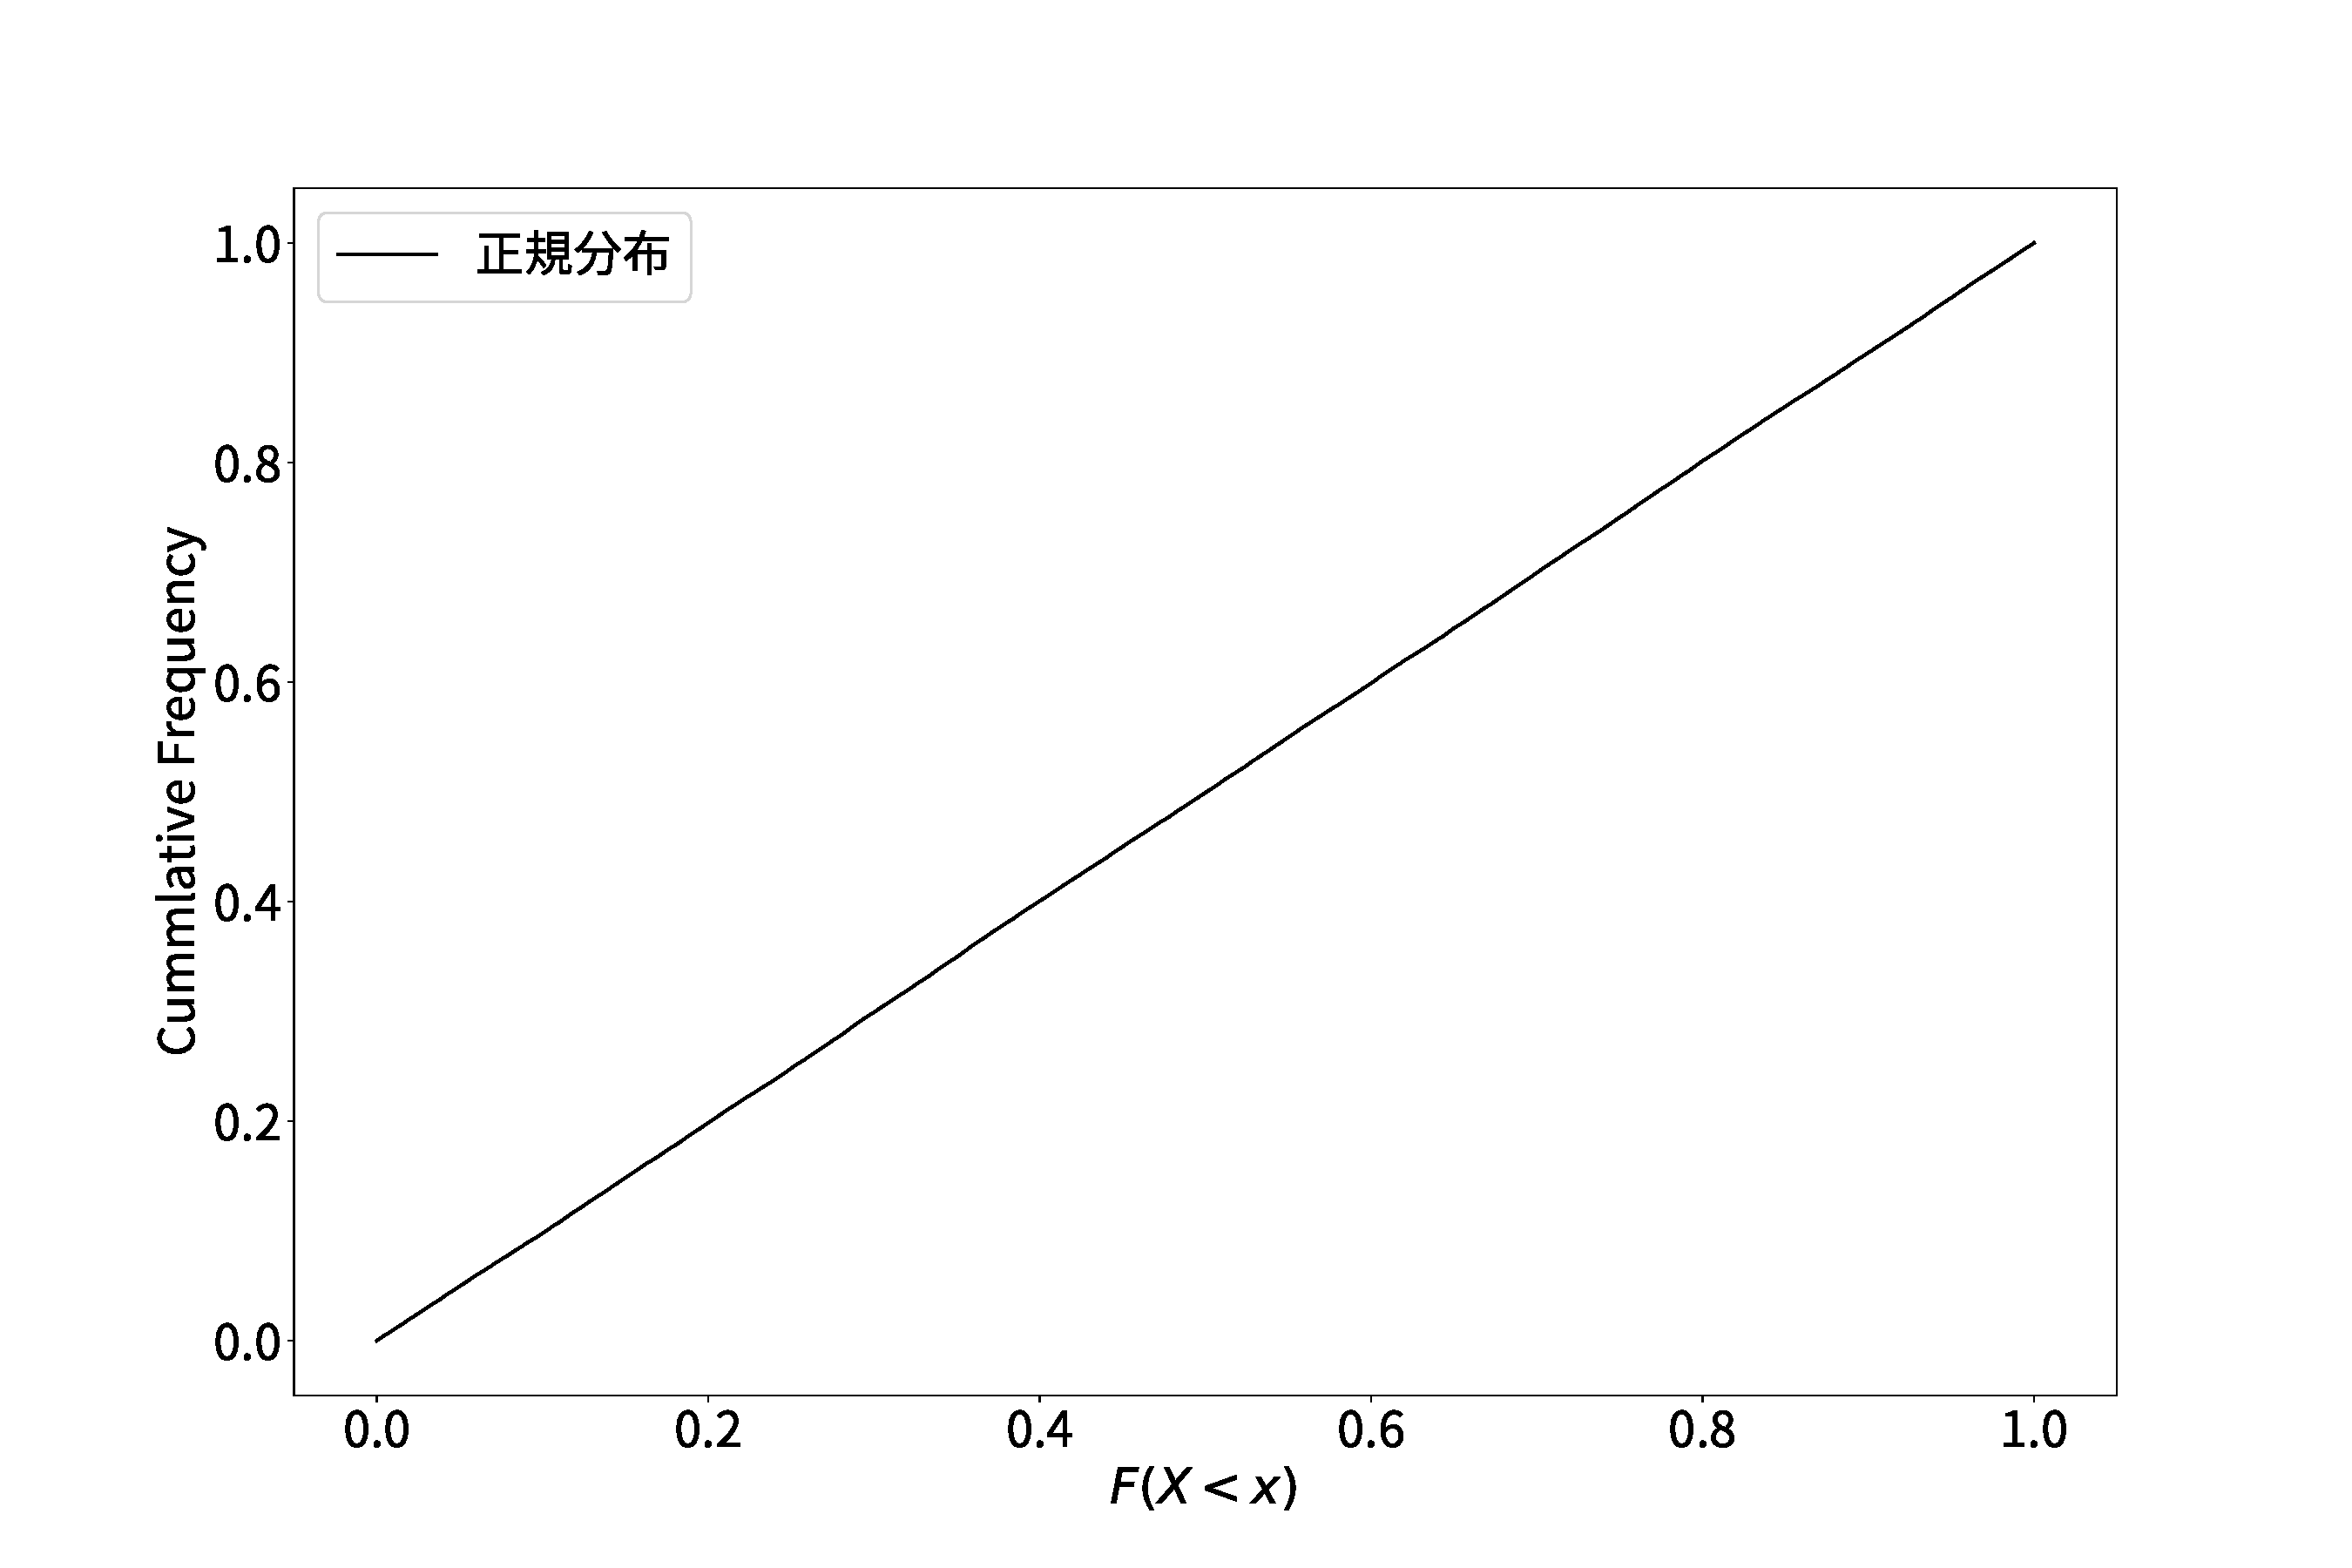
\includegraphics[width=15cm]{./image/04_/test_cummlative_distribution.pdf}
    \caption{累積分布}
   \label{fig:test_cummlative_distribution}
    \end{center}
\end{figure}
%正規モデル$M_N(170,5.8^2)$



\subsection{どんな統計モデルでも$T$統計量で調べよう}
%$\alpha_1$は、統計モデルと、その統計量の関数になっており、言い換えれば、統計量が統計モデルの中で設計通りの振る舞いをしているかを測る指標である。
正規モデルと統計量$T$を使うと、$T$が信頼区間の中にある確率は$\alpha$ である。一方で、指数モデルにおいて、統計量$T$を使った場合、統計量$T$が信頼区間の中にある確率は$\alpha$よりも多くなる。
このことを確かめる。
%ここでは、統計モデルの分布の仮定が正規分布以外の場合においても、$T$統計量を使ってモデルのサンプルを一定の有意水準でモデルの物であるか検証可能かを調べる。
%%このことを数値計算により確かめる。

次の統計モデル$M_E(\lambda)$を構築する。
\begin{enumerate}
    \item $X_1,X_2,\cdots,X_n ,i.i.d\sim F$
    \item $F$は指数分布
    \item 指数分布の母数は$\lambda$
\end{enumerate}
母数$\lambda=1$とした統計モデルを$M_E(1)$とする。
$M_E(1)$からサンプリングした実現値$x_1,x_2,\cdots,x_n$から次の統計量を計算する。
\begin{eqnarray*}
    T &=& \frac{\bar{x}-1}{\sqrt{\frac{\sigma^2}{n}}} \\
 &=& \sqrt{n}\frac{\bar{x}-1}{\sigma}%\sqrt{\frac{\sigma^2}{n}}}
\end{eqnarray*}

正規モデルから得た標本であれば、$T \sim t(n-1)$である。
今回は、指数モデルであるため、$T$値が$t(n-1)$に従わないことで、$p$値の分布に歪みが生じることが予想される。
%しかし、これが成り立つと考えて、計算をおこなうとどのようになるだろうか。

\subsubsection{数値計算}
$T$値が$t(n-1)$の棄却域に入っている頻度を数値計算により計算する。
$M_E(1)$または、正規モデル$M(\mu=0,\sigma^2=1)$からある一定のサンプルサイズの標本を$10^5$回取得する。$T$値を計算し、$T$値より偏った値が得られる確率$p$を計算する。
以下2つの条件において数値計算を行う。
\begin{itemize}
 \item (実験$1$)サンプルサイズを$n=10$とし、$p$値を計算する。その$p$値の分布の偏りを調べる。
 \item (実験$2$)サンプルサイズ$n$を4つの条件$n=(3,10,30,50,100)$とし、それぞれのサンプルサイズ毎に、上で説明した数値計算を行い、$p$が想定している有意水準$\alpha=0.05$を越えない割合を計算する。%($|T|>1.96$となるサンプルの割合)。
\end{itemize}
%以上を数値計算を行なった。

正規モデル$M(0,1)$の場合、$T$値は$t(n-1)$分布に従ので、$p<0.05$となる頻度も、$5\%$程度になることが期待される。
一方で、指数モデル$M_E(1)$の場合、$T$は$t(n-1)$分布に従わない。このことから、実験$1$では、$p$値の分布が偏り、一様分布からずれるそして、実験$2$では、$p<\alpha$となる標本が、$0.05$とは異ることが予想できる。

\begin{figure}
 \begin{center}
  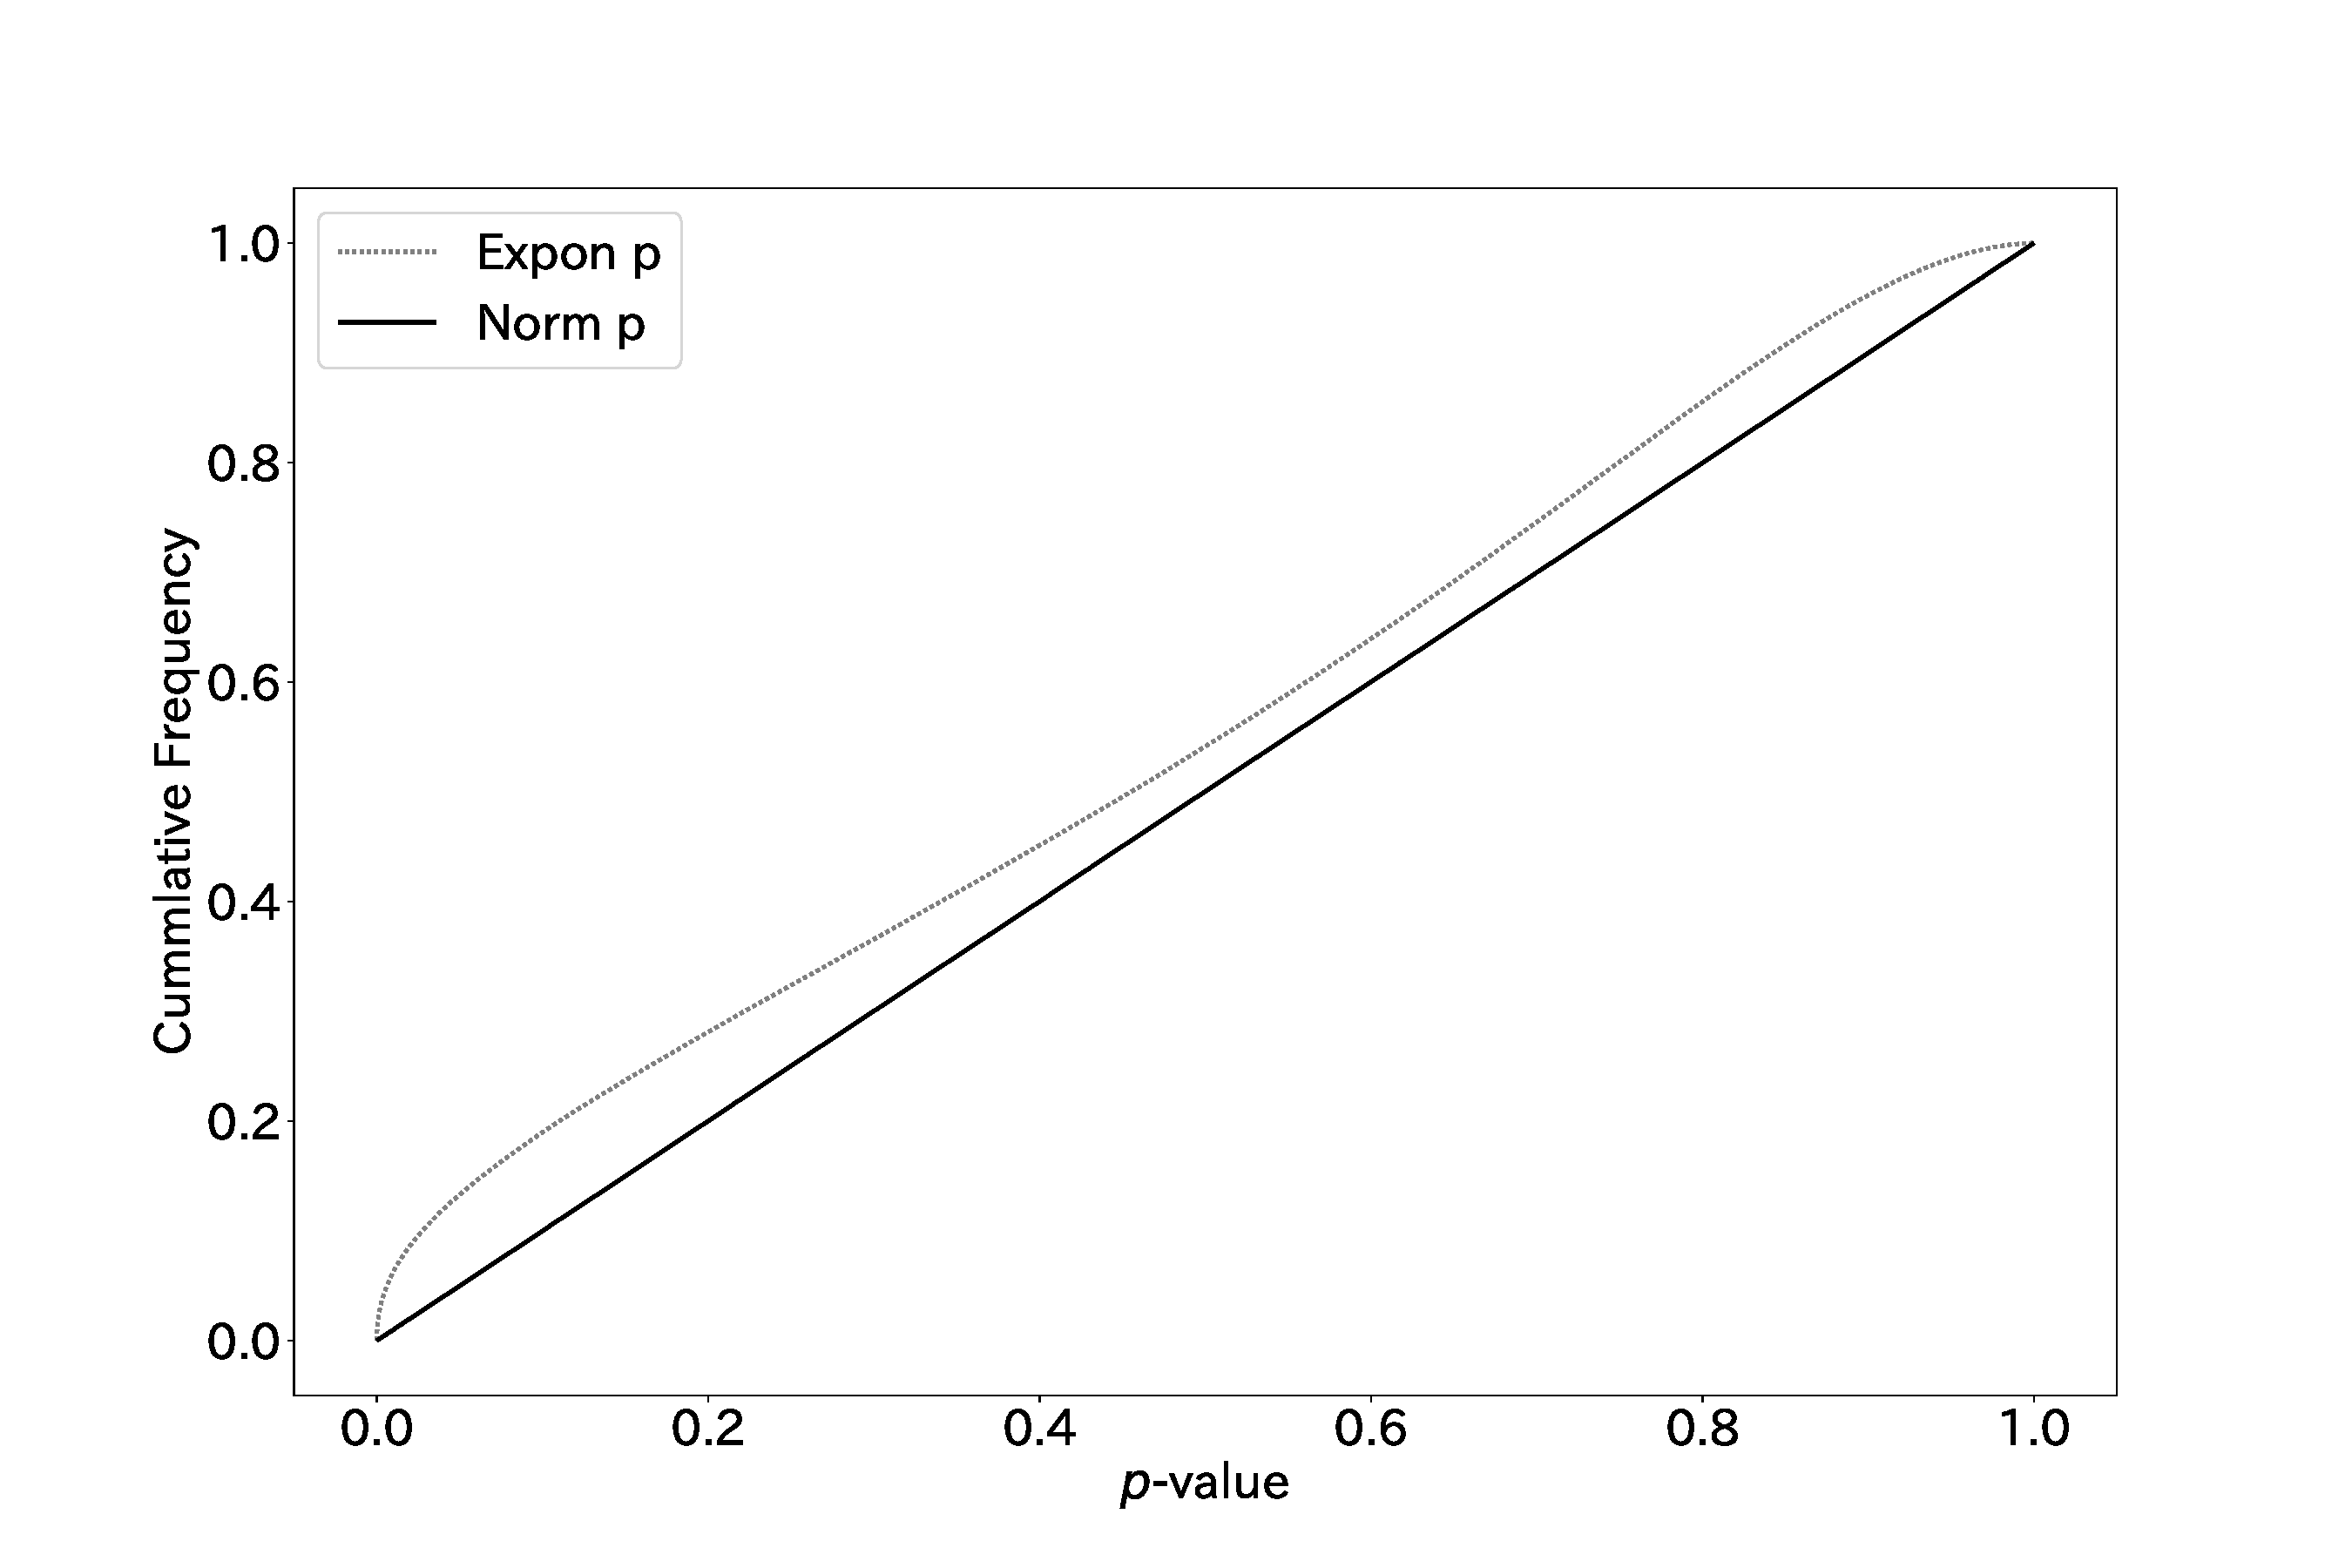
\includegraphics[width=15cm]{./image/04_/N_10_Exponn_T_test.pdf}
 \caption{サンプルサイズ$10$での$p$値の累積分布。実践は、正規モデル。破線は、指数モデル。}
  \label{fig:model_dependent_T_test}
 \end{center}
\end{figure}


\begin{figure}
 \begin{center}
  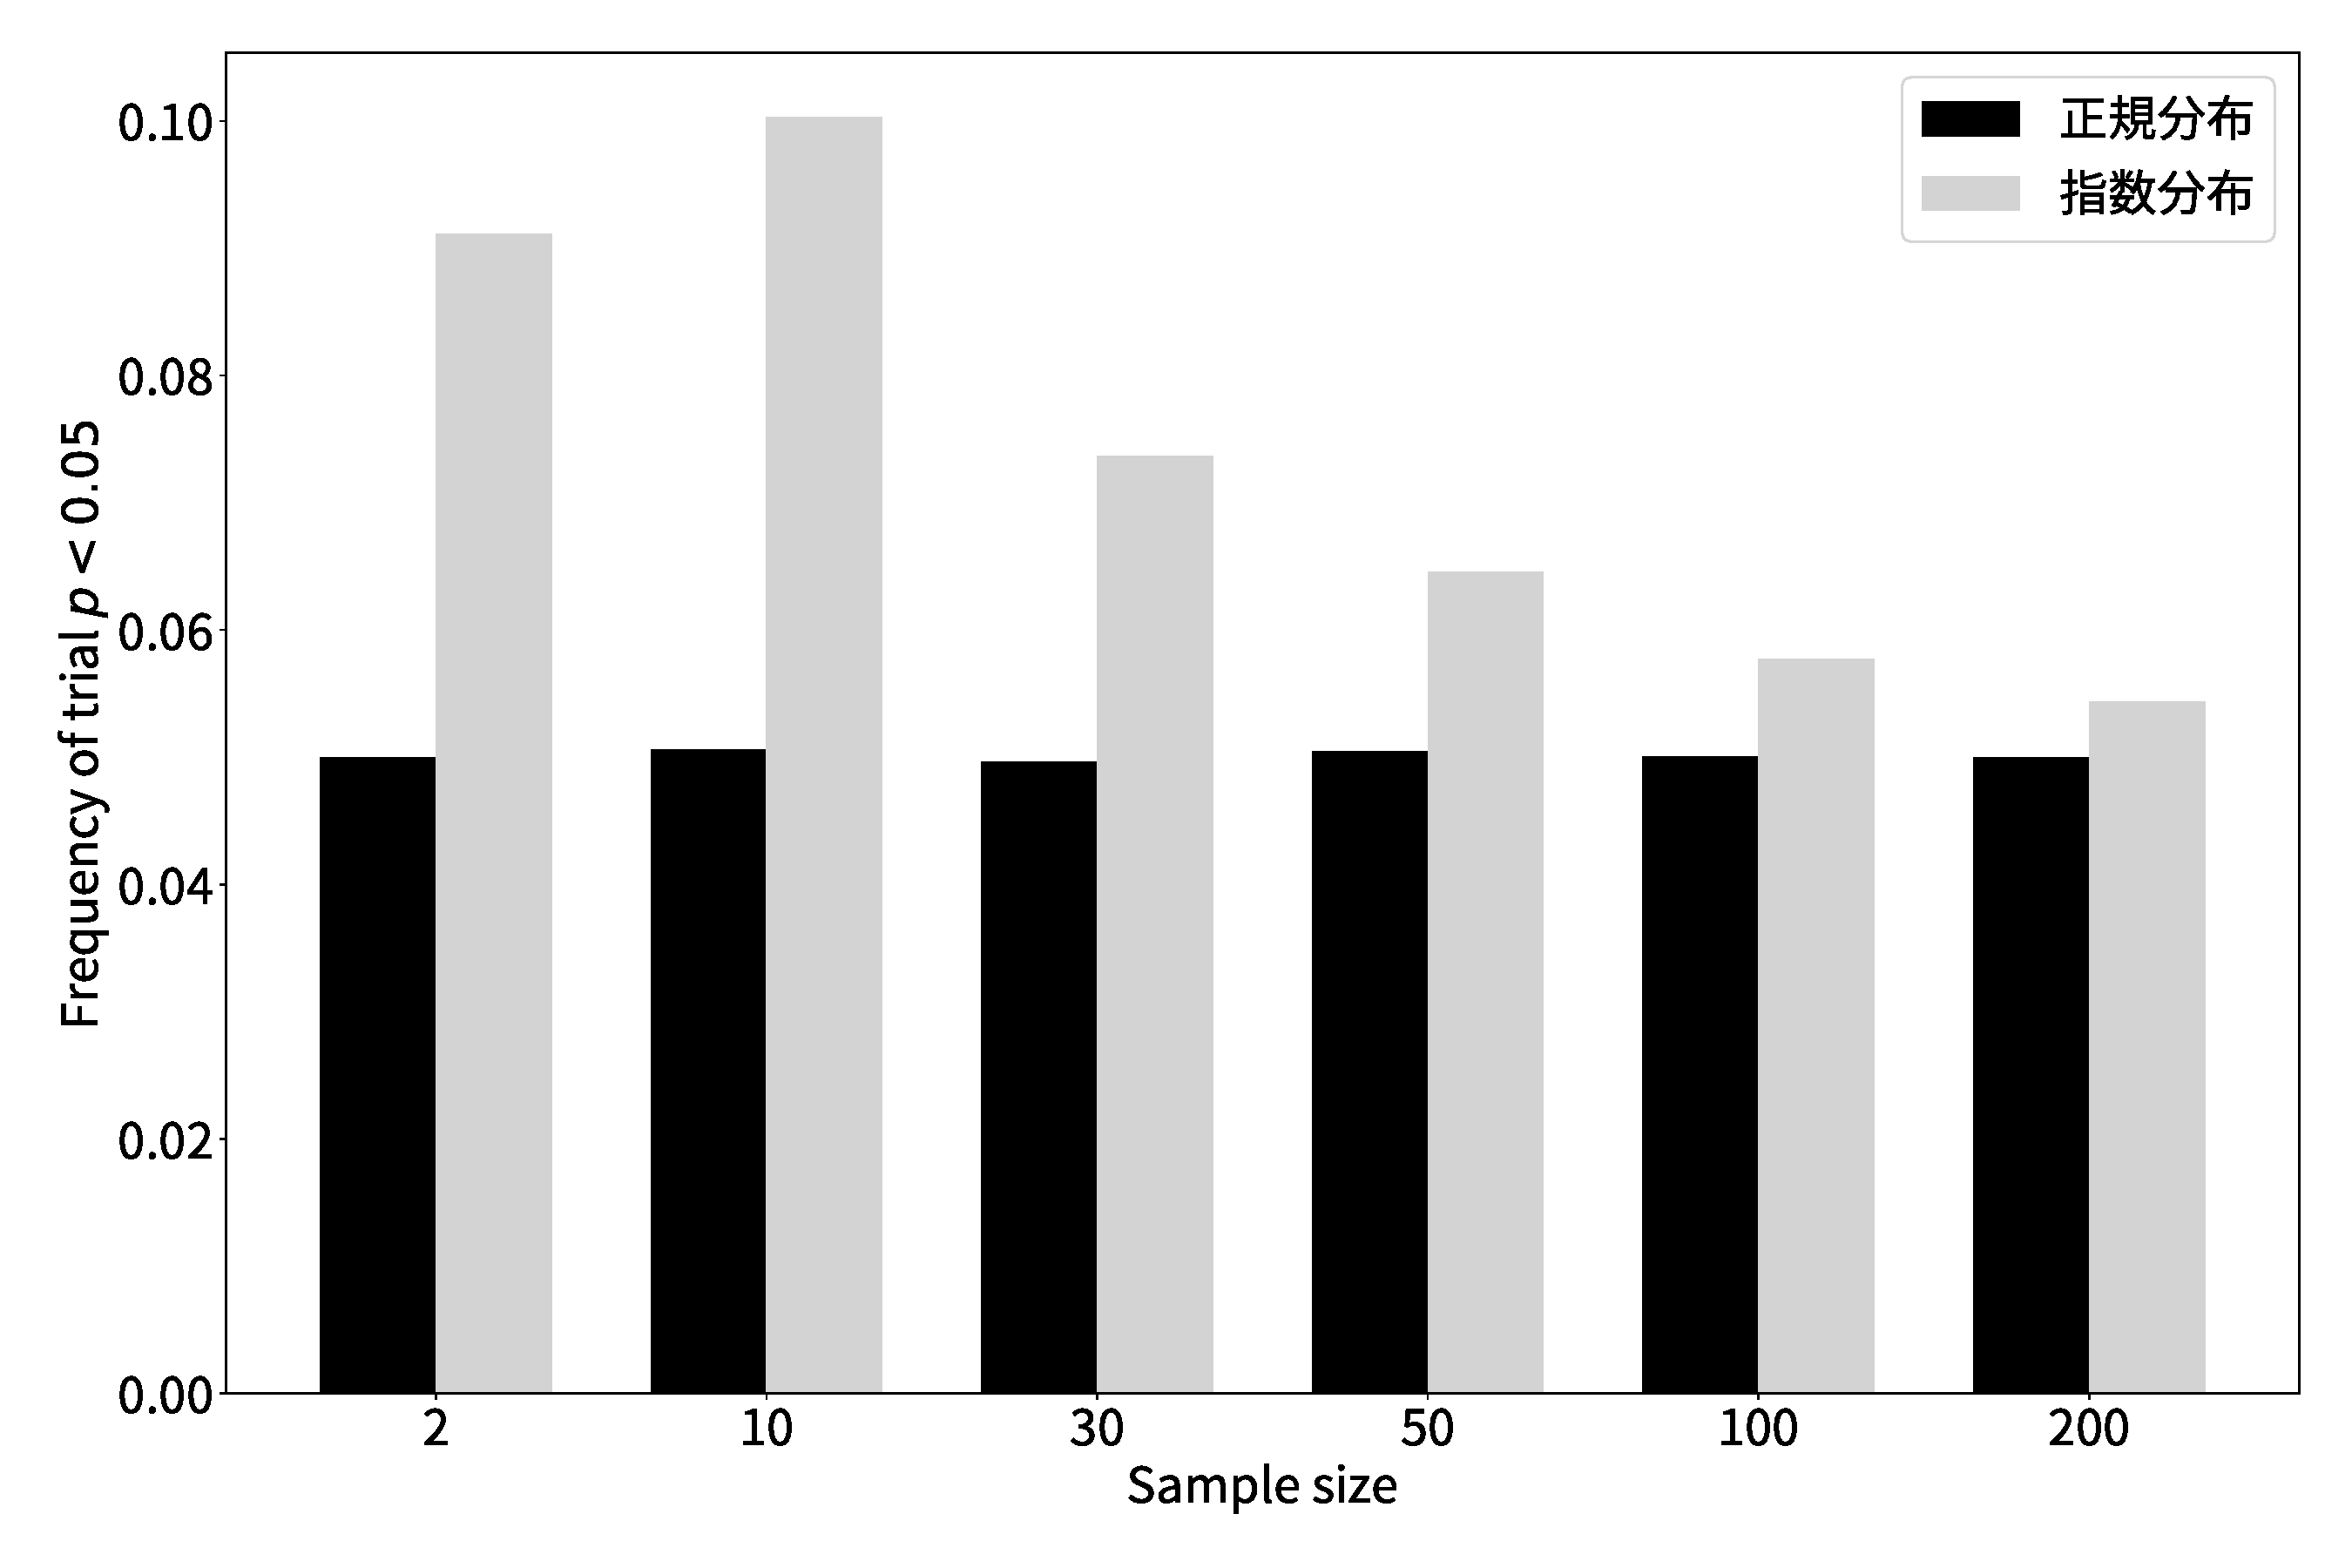
\includegraphics[width=15cm]{./image/04_/expon_T_test_expon_norm.pdf}
%t_test_expon_norm.pdf}
  \caption{それぞれの分布から得た標本の$T$値から計算した$p$値で、$p<0.05$以下になる割合。黒い破線が指数分布での数値計算の結果。灰色の破線が正規分布での数値計算の結果。}
  \label{fig:t_test_expon_norm}
 \end{center}
\end{figure}

実験$1$の結果を図\ref{fig:model_dependent_T_test}に示した。正規モデルであれば、$T$値は正規分布するので、$p$値の分布は一様分布する。$p$値の累積分布が傾き$1$の直線の上にあるので、このことが確かめられる。
一方で、指数モデルにおける$p$値の累積分布は、傾き$1$の直線の上にはないことがわかる。
このことから、指数モデルでは有意水準$\alpha$で検定が行えていない。
%期待した通りのことが起きないことが判った。

実験$2$の結果を図\ref{fig:t_test_expon_norm}に示した。正規分布から標本を得た場合、$p<0.05$になる割合は、サンプルサイズに依存せず、$5\%$程度であり、有意水準$\alpha$で検定が行えている(図\ref{fig:t_test_expon_norm}灰色の点)。
一方で、指数分布から標本を得た場合、$p<0.05$になる割合はサンプルサイズに応じて変化しており、また、どのサンプルサイズでも$p<0.05$となる割合は$5\%$より多い(図\ref{fig:t_test_expon_norm}黒色の点)。

このことから、指数モデルにおいて検定統計量$T$を用いた場合、有意水準$\alpha=0.05$で検定が行えていない。
これは、モデル依存した統計量とそれが従う分布を選ぶ必要があることを示している。
%$p<\alpha$としても、$p>0.05$であることがわかり、統計量を正しく選ばなかったことで、自己否定の過誤がとがわかる。

\if 0 
これはいらない
\begin{SMbox}{サンプルサイズがxx以上あるから$t$検定}
        サンプルサイズがある値以上あるので、中心極限定理により、$t$検定が利用できるというものもある\footnote{http://id.ndl.go.jp/bib/024660739}。このロジックが読み込めなかったので、その謎を明らかにすべく我々はアマゾンの奥地へ向かった。

        %サンプルサイズが1以上であれば、$t$検定を行うことは原理的には可能である。
        データが指数分布的であるときに、$t$検定を使うときに生じる問題は上でみた通りであり、$p<0.05$となる標本の割合が多くなっているので、間違った推測をする可能性が高くなる。
        他の分布関数でもおそらく同じような現象が現れる。
        このことから、我々は「$t$検定が利用可能である」は正確ではなく、「$t$検定を使うことができるが、間違った推測である確率が高くなる」ということだと推察した。

        %サンプルサイズが大きくなれば、$\alpha_1$は小さくなる。
        業界によっては、サンプルサイズが$xx$以上であれば、過誤を無視して良いというふうに言われることもある。実際には、設計したモデルと
\end{SMbox}
\fi
 
\subsection{検定を繰り返し使おう}
%ここまでは、一つの標本に対して、統計モデル$M(\mu)$により推測できるかを考えていた。
%ここでは、$\sigma^2=10^2$とした正規モデル$M(\mu)$によって複数の標本について推測できるかを仮説検定を指標にし考える。
%ここでは、複数の標本について、$M(\mu)$により推測できるかを
正規モデル$M(\mu)$において、$100$個の標本を集め、それらの統計量が信頼区間に入っているかどうかを調べると、およそ$100\alpha$個については信頼区間の外にある。
ここで、標本を得るたびにその統計量が信頼区間にあるかどうかを調べてみると、やはり$100\alpha$個が信頼区間のなかにある。

これを拡張し、二組の標本ペアを100個得て、それらの中で少なくとも1つの検定統計量が信頼区間の中に入っているのは$100\alpha$個程度だろうか。
言い替えると、標本ペアに対して有意水準$\alpha$の検定が行えているだろうか。
%言い替えると、標本ペアのうち、うち少なくとも一つの標本の検定統計量は信頼区間に入っていないなら、正規モデルの標本ペアではないと判断する。
%具体的には、正規モデル$M(\mu)$において、複数の標本が信頼区間に入っているかをたしかめ、それらが正規モデルのサンプルであると考えることができるだろうか。


このとき、それぞれの標本の統計量$T$が信頼区間に入っている確率は、$(1-\alpha)$である。ふたつの標本の統計量$T$が信頼区間に入っている確率は、その積$(1-\alpha)\times(1-\alpha)=(1-\alpha)^2$である。
一方で、棄却される確率$p'$は、$1-(1-\alpha)^2$である。

\begin{table}[hbtp]
    \caption{標本数に応じた$p'$}
    \label{table:multiple_test_reject_prob}
    \centering
    \begin{tabular}{lcr}
      \hline
      標本数  & $\alpha=0.05$  &  $\alpha=0.01$ \\
      \hline \hline
       1 & $0.05$  & $0.01$ \\
       2 & $0.0975$ & $0.0199$\\
       3 & $0.142$ & $0.0297$\\
       4 & $0.185$ & $0.0394$\\
    \end{tabular}
  \end{table}
表\ref{table:multiple_test_reject_prob}は、標本数に応じた$p'$である。標本数が大きくなるについれて、$p'$が大きくなることがわかる。
これは、標本の組み数が多いと、標本がモデルのものではないと判定されやすくなることを示している。

%$\alpha_1$がレベル$\alpha$の検定になっていない場合、$\alpha_2$はさらに有意水準$\alpha$から隔たりの多い数値になる。

\subsubsection{数値計算}
具体的に数値計算を行う。サンプルサイズ$10$の標本を$4$つ(標本数$4$)得る。
この試行を$10^6$回繰り返す。
各試行において、すくなくとも一つの標本の$p$値が有意水準$\alpha$を超ていることを確かめる。

具体的に以下のコードを実行すればよい。
最後の行で、1から有意水準を超ていないサンプルの割合をひいて、少なくとも一つは有意水準を超ていた試行の割合を計算している。
\begin{lstlisting}
repeats =10**6
sampleN = 4
N = 10
alpha = 0.05
mu=170
sigma = 5.8
sample = norm(mu,sigma).rvs(size=(sampleN,N,repeats)) # sample.shape = (sampleN, N , repeats)
normal_sample = np.sqrt(N)*(np.average(sample,axis=1).T-mu)/sigma # normal_sample.shape = (repeats, sampleN)
p_values = norm.cdf(normal_sample)
flag = (p_values < alpha*0.5)|(p_values > 1-alpha*0.5)
1-(np.sum(np.sum(flag,axis=1) == 0))/repeats
\end{lstlisting}
結果は、およそ$0.1849$程度になり、解析解と一致することがわかる。

\subsection{最小の$p$値を採用しよう}
固定のサンプルサイズの標本をいくつか得て、それぞれの標本において$p$値を計算し、その中で最小の$p$となるものを採用するという操作を数値実験により行った。
具体的には、平均分散をそれぞれ$\mu=170,\sigma^2=5.8^2$とし、正規分布からサンプルを生成した。
またサンプルサイズを$N=10$とし、標本のペア数を$2$とした。それぞれのサンプルにおいて$p$値を計算し、$p$値の中で最小の$p$を採用した。
これを$10^3$回繰り返した。

\begin{lstlisting}
repeats =10**6
sampleN = 4
N = 10
alpha = 0.05
mu=170
sigma = 5.8
sample = norm(mu,sigma).rvs(size=(sampleN,N,repeats)) 
normal_sample = np.sqrt(N)*(np.average(sample,axis=1).T-mu)/sigma
p_values = norm.cdf(normal_sample)

min_p_values = np.min(p_values,axis=1)
first_p_values = p_values[:,0]
\end{lstlisting}

図\ref{fig:minimum_p_value_choice}には、数値計算の結果を示した。
標本がペアではないなら$p$値は一様分布するので、累積分布は傾き$1$の直線の上にのる。数値計算でも同様の結果が示されている。
一方で、最小の$p$値を選択すると、図\ref{fig:confidence_interval_model}に示したように、傾き1の直線の上に乗らない。
これは、$p$値が一様ではなく、$p$値が小さなものが通常よりも大きな頻度で生じていることを示唆している。
このことから、有意水準$\alpha$を定めると、$p<\alpha$となる$p$値は$\alpha$よりも大きな頻度で生じており、
有意水準$\alpha$で検定ができないことが示される。

\begin{figure}
  \begin{center}
    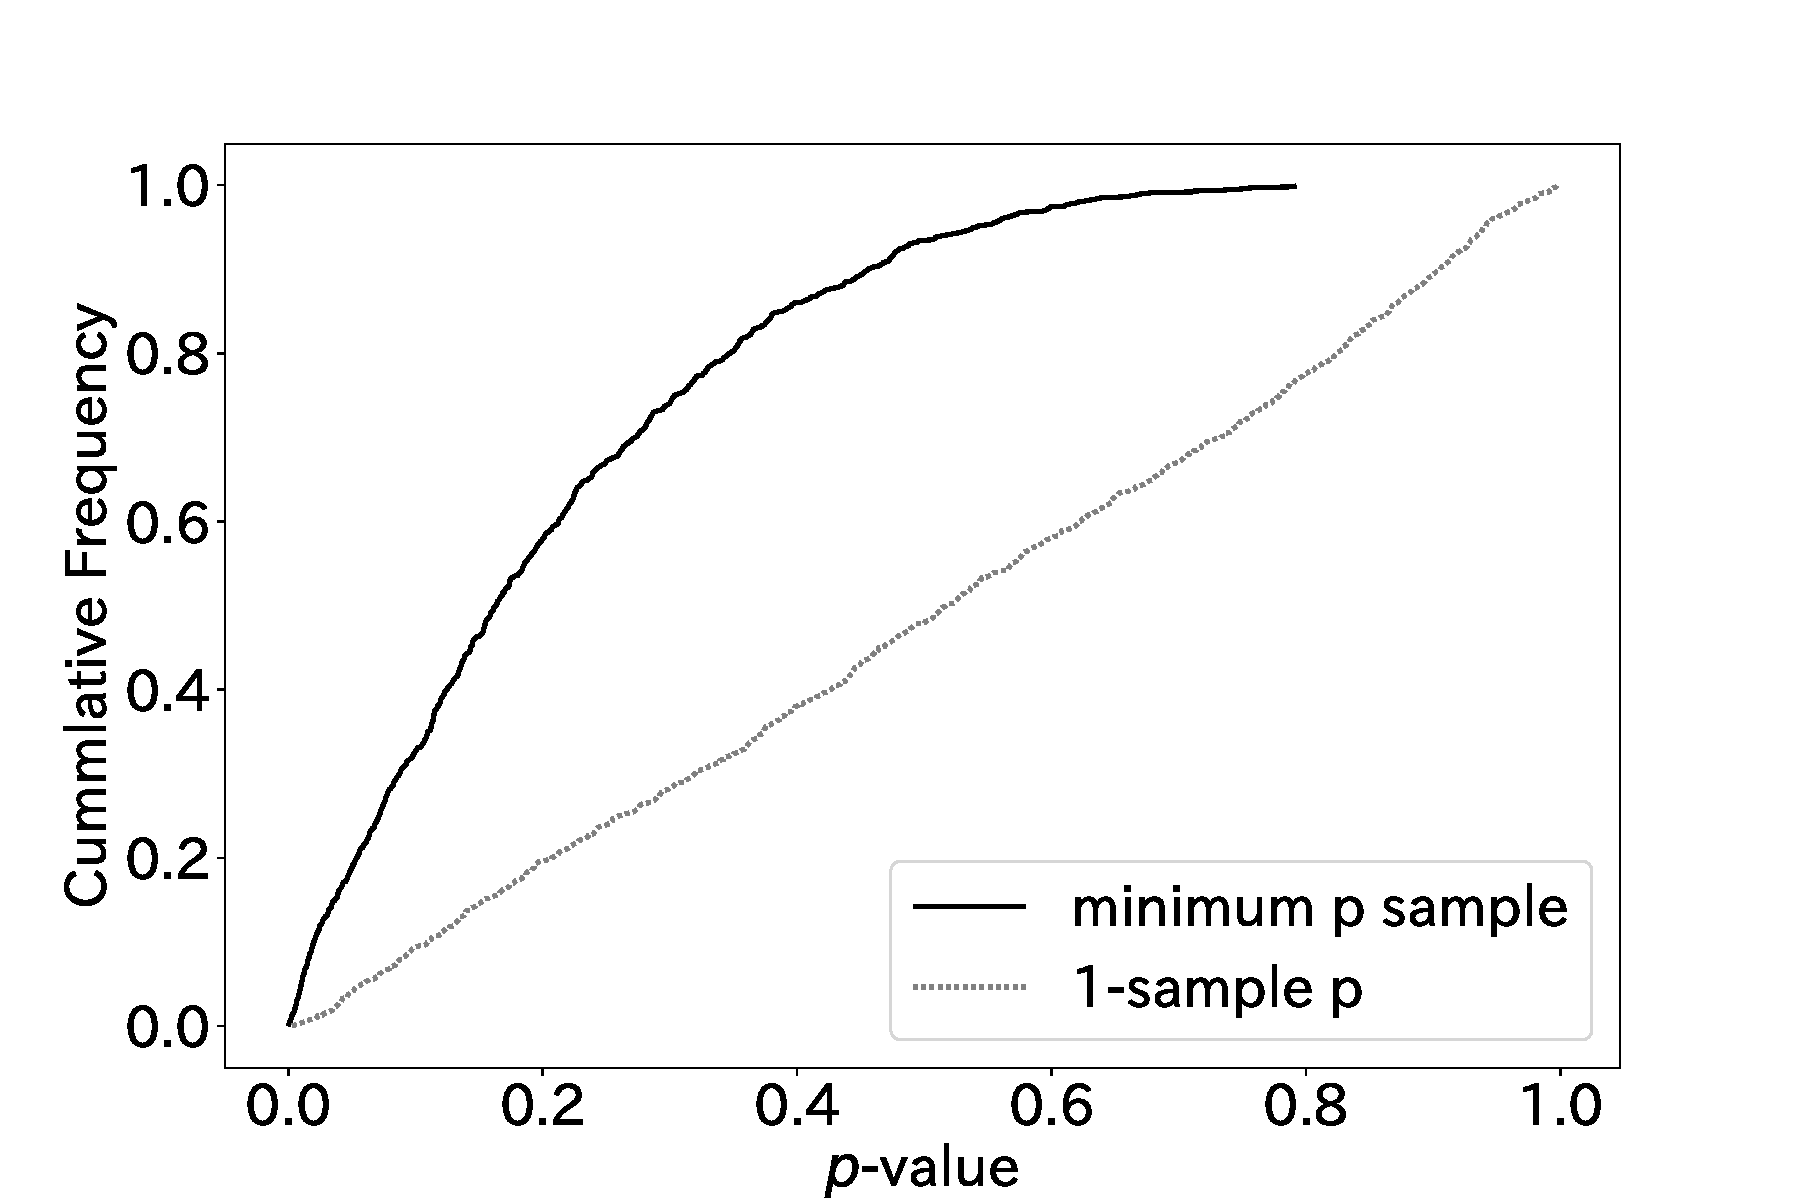
\includegraphics[width=15cm]{./image/04_/Minimum-p-values-choice-exmepriment.pdf}
    \caption{最小の$p$値を採用したときの累積分布。実線は2つの標本の中から最小の$p$を選んだときの累積分布。破線は一つのサンプルから$p$を計算した場合の累積分布}
        \label{fig:minimum_p_value_choice}
    \end{center}
\end{figure}

\subsubsection{多重検定との関係}
この処理は一つ前の節で説明した多重検定と一致する。
具体的には、すくなくとも一つの標本において$p<\alpha$となるは、ペアの中で最小の$p$値を採用すると同じである。
このことを数値計算により確かめておく。
\begin{lstlisting}
repeats =10**6
sampleN = 4
N = 10
alpha = 0.05
mu=170
sigma = 5.8
sample = norm(mu,sigma).rvs(size=(sampleN,N,repeats))
normal_sample = np.sqrt(N)*(np.average(sample,axis=1).T-mu)/sigma
p_values = norm.cdf(normal_sample)

np.sum(np.min(p_values,axis=1)<alpha)/repeats
\end{lstlisting}
結果は、$0.184$であり、解析解\footnote{解析解という用語は正しいのか不明}と一致する。



\subsection{サンプル追加による$p$値の変化}
標本にサンプルを追加しながら検定をおこなうと、期待している結果が得られるだろうか(\cite{simmons2016false})。標本に、サンプルを追加する毎に検定を実行する。
この試行を複数回繰り返し、一度でも有意水準を下回った標本の個数を数える。
ただし、$p<\alpha$になるまで繰り返すと必ず有意となるので、最終的なサンプルのサイズはあらかじめ決定しておく。

以下の数値実験を行う。
初期サンプルサイズを$N=10$または$N=20$、最終サンプルサイズ$N_{max}=50$、標本数$10^6$とした。サンプルを$\Delta s$個追加し、検定を実行した。
$\Delta s$は、$1,5,10$または$20$とした。それぞれの$\Delta s$に応じた検定回数は$41,9,5,3$回である\footnote{多重検定とは条件が異なるので、$\Delta s=41$だとしても、$p<\alpha$となる頻度が$1-(1-\alpha)^{41}$とならない。}。


図\ref{fig:multiple_test_additional_sample}が数値実験の結果である。
サンプルサイズを追加する毎に検定をすると、$p<\alpha$となる頻度が$\alpha$以上になる。このことは、有意水準$\alpha$の検定が行えないことを示している。
%どの場合においても$p<\alpha$となるのは$\alpha$程度であってほしいが、これは数値実験の結果と一致しない。

\begin{figure}
  \begin{center}
    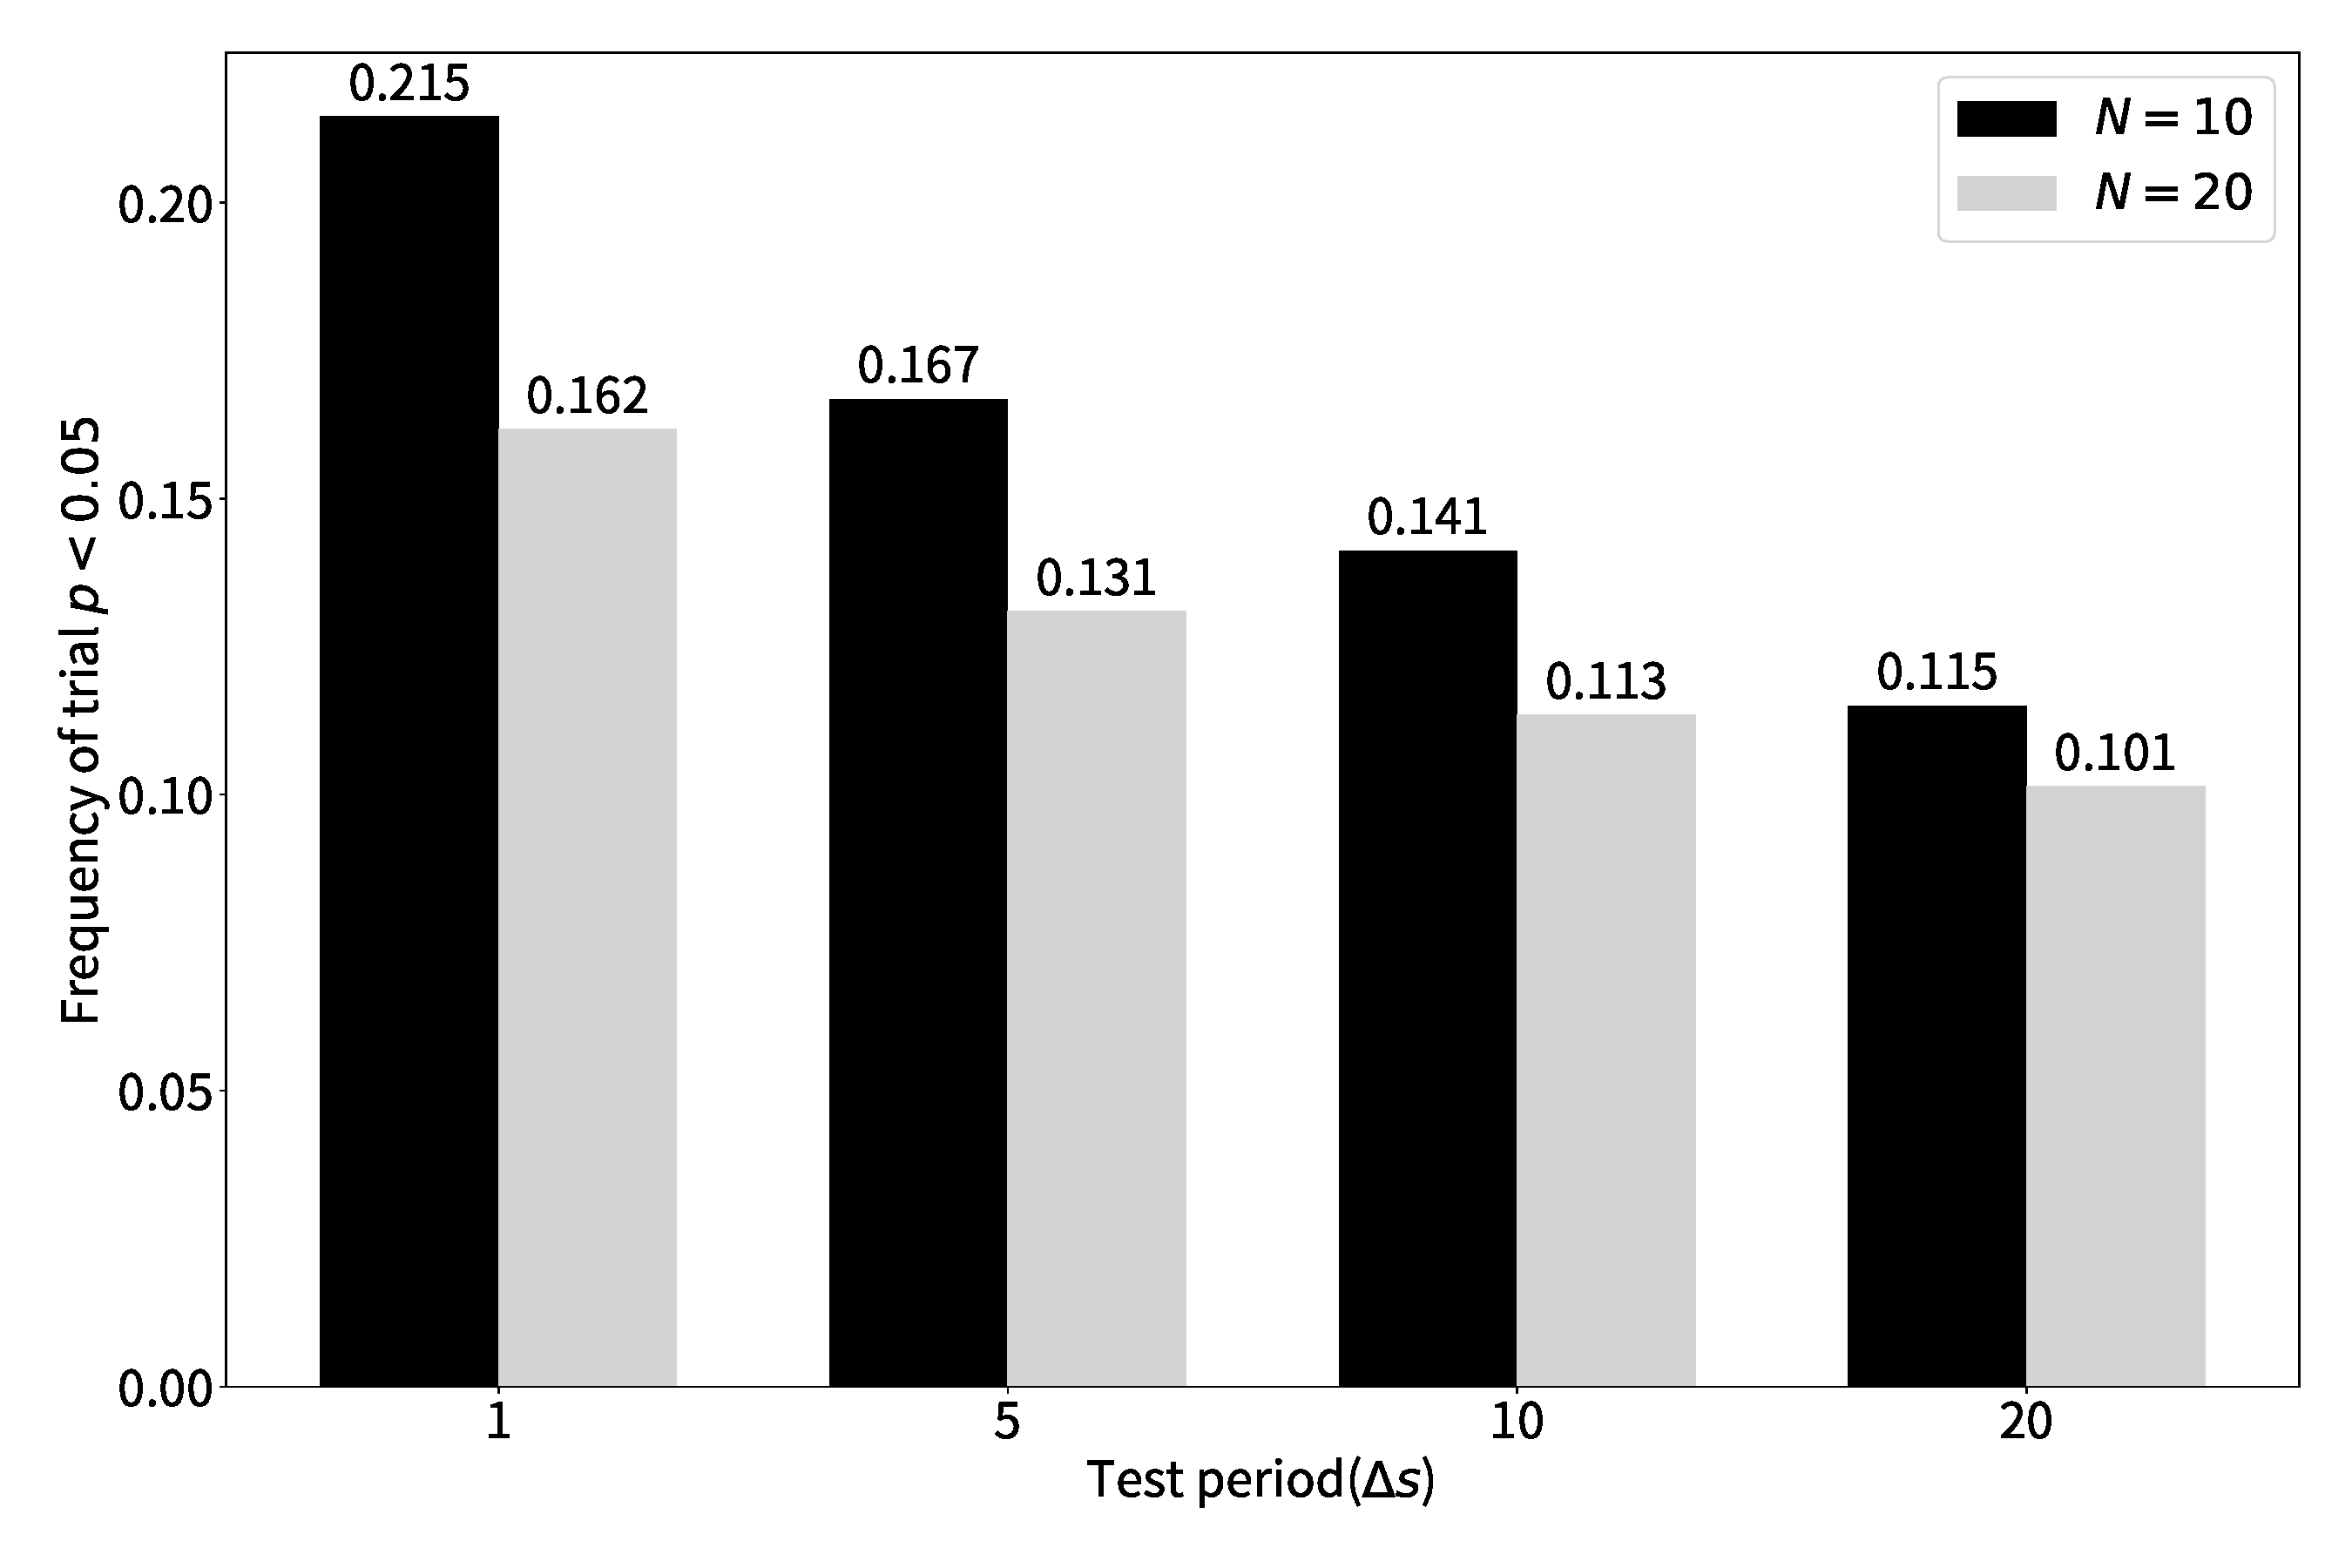
\includegraphics[width=15cm]{./image/04_/multiple_test_additional_sample.pdf}
    \caption{サンプルの追加個数と検定を実行。サンプルの追加個数を$\Delta s$としその違いによる$p<0.05$となる頻度。初期サンプルサイズが$10$(黒色)と$20$(灰色)。}
        \label{fig:multiple_test_additional_sample}
    \end{center}
\end{figure}

以下に数値実験用のコードを残しておく\footnote{わかりにくいコードになってしまった。後で書き換えたい。}。
\begin{lstlisting}
sampleN = 10**6
N = 10
maxN = 50
mu = 170
sigma = 5.8

delta = 1

def nan_index(N,maxN,delta):
    index = np.array([~(np.arange(maxN)>=i) for i in np.arange(N,maxN+delta,delta)] )
    nan_index = np.ones(index.shape)*index
    binary_index = index.astype(np.float64)
    binary_index[~index] = np.nan
    return binary_index

def stopping_rule(delta):
    nan_array = nan_index(N,maxN,delta)
    sample_num = np.count_nonzero(~np.isnan(nan_array),axis=1)


    # sample
    norm_ = norm(mu,sigma)
    sample = norm_.rvs(size=(sampleN,maxN))

    rep_sample = np.tile( sample.reshape((-1,1,maxN)), reps= (len(nan_array),1))
    restrict_sample = rep_sample*nan_array
    sample_mean = np.nanmean(restrict_sample,axis=-1)

    Z = np.sqrt(sample_num)*(sample_mean-mu)/sigma
    p = norm.cdf(Z)
    p_ = ((p < 0.025) | (p>0.975))
    true_once = (np.cumsum(p_,axis=1)>=1)
    return np.sum(true_once[:,-1])/sampleN
N = 10
result_10 = [stopping_rule(delta) for delta in [1,5,10,20]]
\end{lstlisting}

\subsection{いつかは有意になる}\label{large_sample_size_significant}
非常にわずかなモデルのちがいでも検定を使うと、モデルの標本ではないと言えてしまうことを確認する。
まず、二つの正規モデルを構築する$M_a=M(170,5.8^2),M_b=M(171;5.8^2)$とした。
母数平均が殆ど一致していることを、母数平均の$\sigma$規格化量$D$を計算することで確認しておく。
\begin{equation*}
 D=\frac{|\mu_a-\mu_b|}{\sigma} = 1/5.8=0.172
\end{equation*}
これらのモデルはほぼ同じような予測を行うことは理解できる。
%この$D$が小さいか大きいのかはモデルだけでは判断できない\footnote{データとの比較をするさいは重要な量の一つである}。ただ、きるだろう。

モデル$M_a$において生成したサンプルがサンプルサイズを大きくすることで、$M_b$において検定統計量の出現頻度が$p<\alpha$になる様子を確認しておく。
具体的には、$M_a$においてサンプルサイズ$300$の標本を10個生成する。
それぞれの標本において、サンプルサイズを$1\sim 300$までにし、それぞれのサンプルサイズにおける$p$値を計算する。

\begin{lstlisting}
def nan_index(N,maxN,delta):
    index = np.array([~(np.arange(maxN)>=i) for i in np.arange(N,maxN+delta,delta)] )
    nan_index = np.ones(index.shape)*index
    binary_index = index.astype(np.float64)
    binary_index[~index] = np.nan
    return binary_index

def calc_p():
    maxN = sample_size
    nan_array = nan_index(1,maxN,1)
    sample_num = np.arange(1,maxN+1)
    norm_ = norm(mu_a,sigma)
    sample = norm_.rvs(size=(sample_size,num_of_sample))

    rep_sample = np.tile( sample.reshape((-1,1,maxN)), reps= (len(nan_array),1))
    restrict_sample = rep_sample*nan_array

    sample_mean = np.nanmean(restrict_sample,axis=-1)
    Z = np.sqrt(sample_size)*(sample_mean-mu_b)/sigma # モデルM_bのサンプルか?
    return Z

nan_array = nan_index(1,sample_size,1)
mu_a=170
mu_b=171
sigma = 5.8
sample_size=300
num_of_sample = 10

Z = calc_p()
\end{lstlisting}

図\ref{fig:time_series_p_value_depends_sample_size}にはサンプルサイズに応じた$p$値を表示した。
サンプルを増やしていくことで、$p$値が徐々に小くなることがわかる。
殆ど同じようなモデルであってもサンプルサイズを増やしていけば、あるモデルのサンプルではないと主張できる。
%このことは、データをモデルを比較するさいに非常に重要な事項である。

\begin{figure}
 \begin{center}
  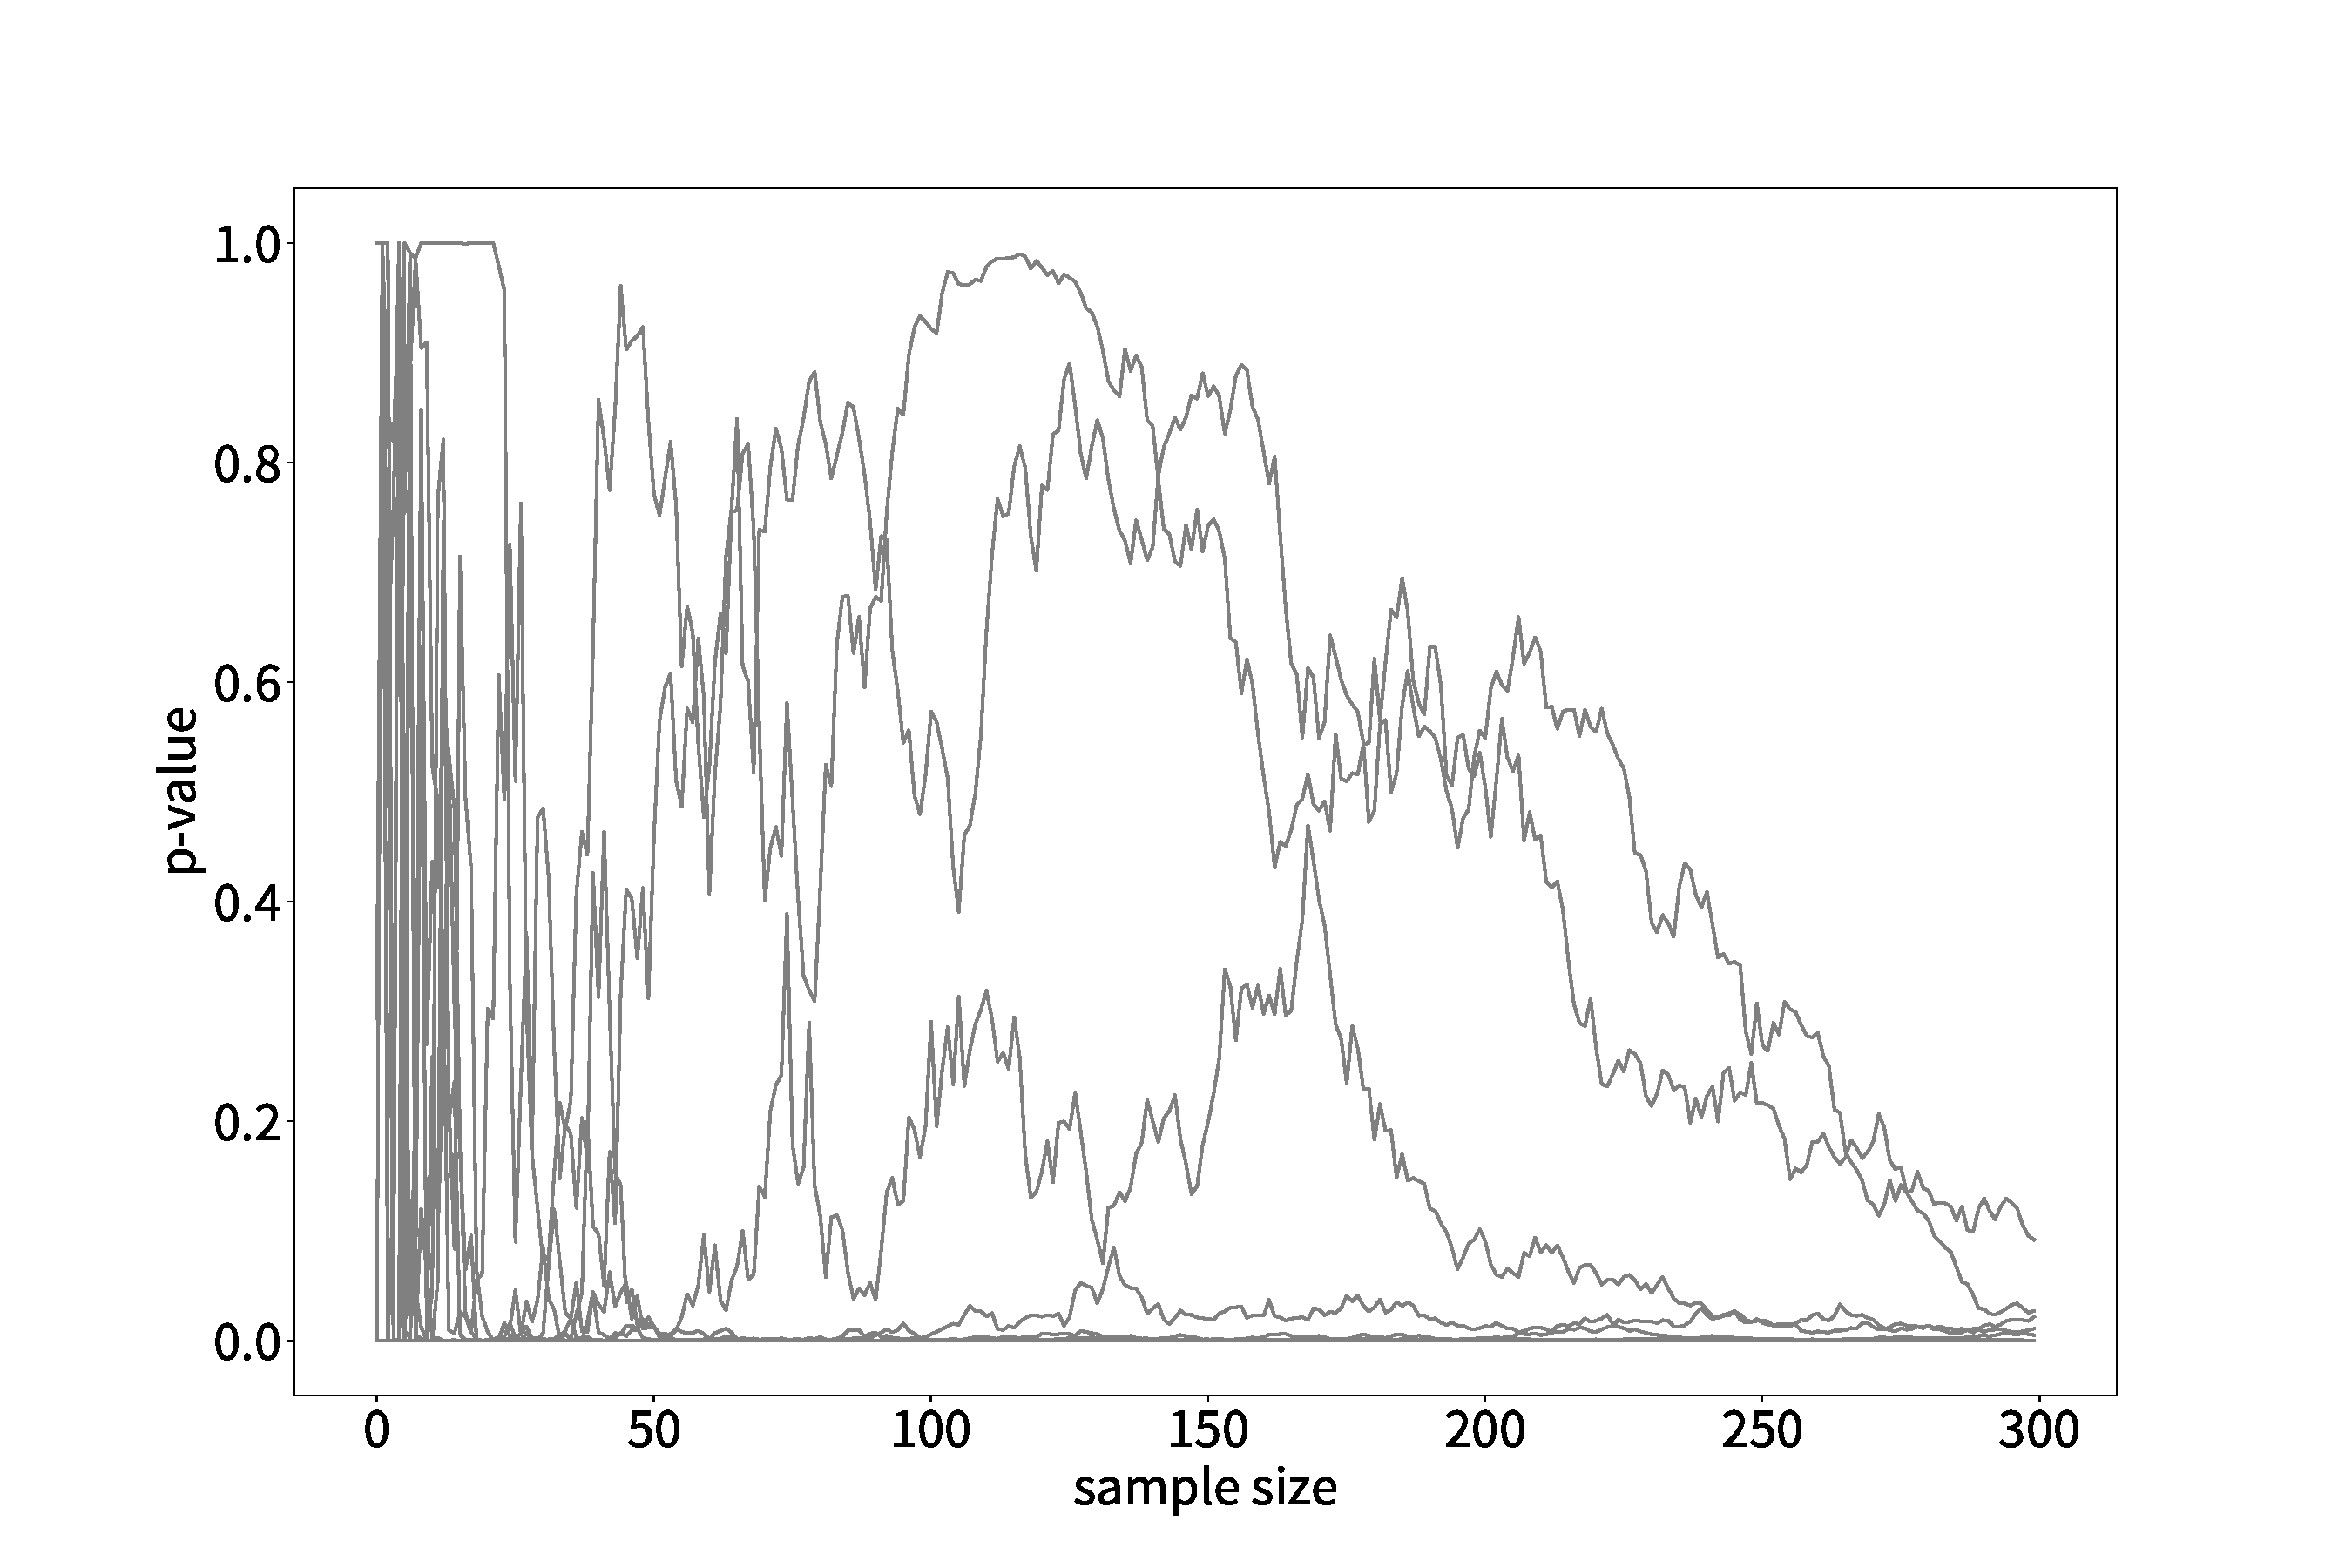
\includegraphics[width=15cm]{./image/04_/p_sample_size.pdf}
  \caption{サンプル応じた$p$値の変化}
  \label{fig:time_series_p_value_depends_sample_size}
 \end{center}
\end{figure}



\subsection{いつかは有意にならない}
ある正規モデル$M_a$において、サンプルを生成し、標本にサンプルを追加し、追加毎に$p$値を計算する。
結果を図\ref{fig:time_series_p_value}に示してある。
この図の通り、サンプルサイズを追加すると、一時的には$p$値があるしきい値(図の点線$\alpha=\frac{0.05}{2}$または$1-\frac{0.05}{2}$)を下回ることがあるが、その後サンプルを加えると、有意水準よりも大きな値となることがある。
よく言われる「検定はサンプルサイズを大きくするといつかは有意水準を下回る」に反する\footnote{こう言われているのは、理論と実験の話を混ぜているためである。正確には、モデルと実験を比較するさいに、実験でサンプルサイズを逐次追加すると、モデルと実際の乖離があきらかになりやすいため、有意になりがちである。既に前の小節で確認した。}。

\begin{figure}
  \begin{center}
    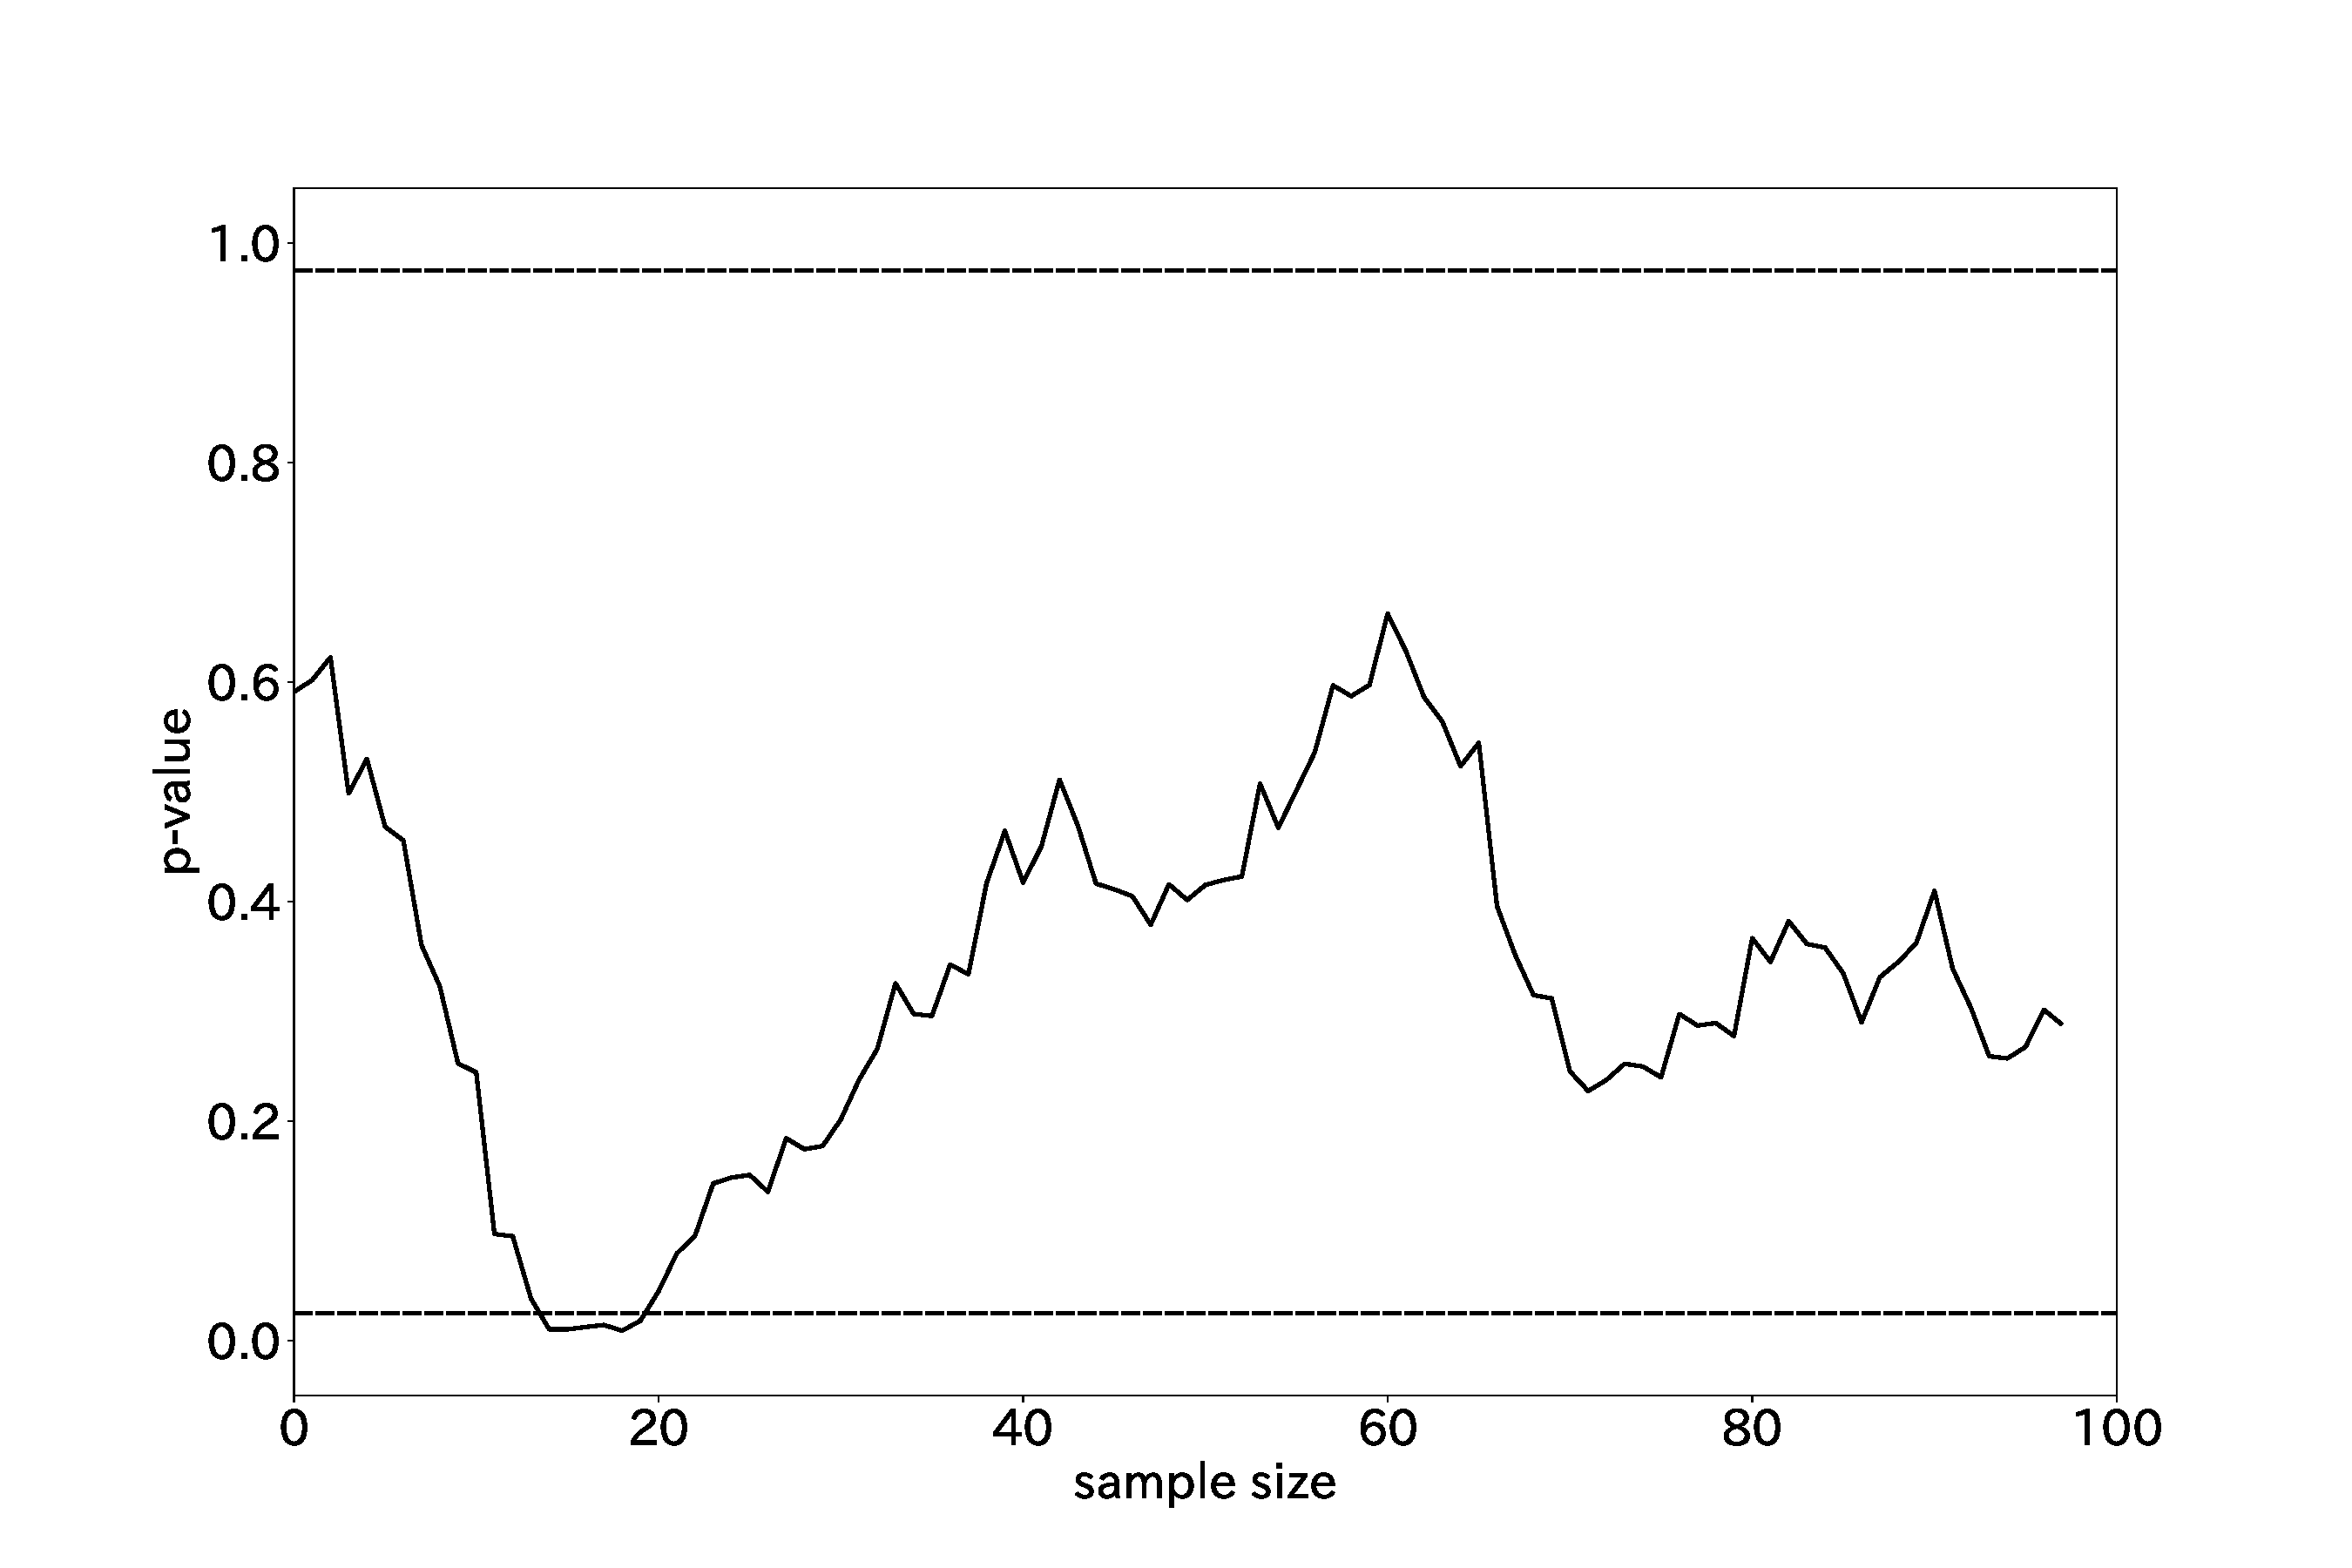
\includegraphics[width=15cm]{./image/04_/recurssive_test.pdf}
    \caption{サンプルの追加に応じた$p$値の変化}
        \label{fig:time_series_p_value}
    \end{center}
\end{figure}





\if 0
有意水準$\alpha$で検定ができていないのは、
\begin{itemize}
  \item 
\end{itemize}
\fi

\begin{comment}
これはむりかも
\section{類似度の誤推定}
統計モデルの間の類似度を検出力といった。
統計モデルに対して、不適切な統計量を与えたとき、検出力を歪める。
これを類似度の過誤といい、その確率を$\beta'$で表す。
直接または数値計算を行い$\beta$を計算することがおそらくできそうだが、面倒なので行わない。
\end{comment}


\subsection{まとめ}
ここまでで、検定統計量から複数の標本のうち$100\alpha\%$程度をはじきだす仕組みを説明した。
また、仕組みを適用するさいに、途中処理を加えてしまうと、事前に決定した有意水準での検定ができないことも明らかになった。
モデルと我々のデータを比較するさいにこれらに注意して解析する必要がある。

%この仕組みでは、ある標本がモデル由来かどうかを調べることはできない。
%論文統計では、多重検定には注意をはらうが、他の検定操作については気にとめていないことが多い。%特に、検定まえ検定が非難されるのは、まずは検定では何もわからないという点で、次に多重検定の問題がある。

%母集団から得たデータはモデルから生成されていると考えることができないし、母集団から得た標本の$100\alpha\%$を検出することが目的ではない。
%我々が考えている系は統計的仮説検定の前提と異っており、モデル上で生じる事象と現象とを同一視できない。
%このことから、データとモデルを比較するさいには、これらの点について考慮することが必要となる。




\section{データとモデルの比較}
ここで、いくつかのことを定義しておく。
\begin{defi}
    統計モデルと標本を比較して、モデルが母集団のことを予測できないとさまざまな指標をもとに判断するとき、統計モデルを却下すると宣言する。
    %ある標本から求められた統計量以上に大きな値が得られる確率を$p$値と呼ぶ。
    %絶対にダメと判断されないときは、統計モデルを採択(棄却の対義語)すると宣言しない。
    %統計モデルが棄却されるのは、統計モデルの仮定によって変化する。本書の範囲内であれば、統計モデルの母数、分布関数、独立同一の分布関数からサンプリングされたことによる。
    %最尤統計モデルにおいて、棄却されない統計モデルの母数の範囲を信頼区間といい、棄却されるモデルの母数の範囲を棄却域という。
\end{defi}
%ある閾値$\alpha$を決めて、それよりも小さな$p$値をもつ標本について、モデルから得られたものではないと判断する。ここで、$\alpha$を有意水準という。

\begin{SMbox}{検定統計量や$p$を計算するだけで解析完了}
 データとモデルの乖離具合を示す指標を計算するだけになってしまう。
 標本がモデルにより推測可能かを調べることで、より多くの予測を引き出すことができる。
 また、検出力$\beta$やサンプルサイズ、中心間の距離の規格化量$D$も記載すればいいということではない。
\end{SMbox}


ここで、母集団から無作為抽出した標本(モデルから生成された標本ではない)を正規モデルにより、予測できるかを考える。
すでに議論したように、標本から検定統計量を計算し、検定統計量よりも偏った値が出現する確率($p$値)を計算する。
$p$値が小さければ、モデルにより予測できないかもと疑い、値が$0$から遠いほど、もしかしたらモデルで予測できるのかもしれないと疑う\footnote{$p$値だけで判断してはいけない}。
%標本を元に、モデルにより予測できなさそうかを考えている。
%このとき、モデルを却下すると宣言する。
%$p$値が$\alpha$よりも小さいとき、流石にこのモデルでは予測できないでしょうと判定する。
%$p$値が$\alpha$よりも大きい場合でも、そのままこのモデルで予測できるとは宣言しない。他の指標やデータとモデルをグラフにより比較し、予測できそうかを考察する必要がある。

%この標本は、モデルからサンプリングしたものではない。
%標本の統計量が、モデルの上で得られやすいものかを調べる。
%$M_a$を棄却する判断をする閾値は、言い換えると、統計モデル$M_a$の棄却される母数(棄却域$R$)の出現確率を$\alpha$とした。

以上のことは、托卵行動に例えることができる\footnote{ピーと鳴く鳥に$p$値を例えたお話を作りだすことが目的で特に意味はない。将来的には以下の文章は消そう。}。
モズは、カッコウに対して卵を託す托卵を行い、カッコウは、モズの卵とは気が付かず、そのまま育てる。
ここで言い換えたいのは、カッコウは統計モデルであり、卵は標本そして、モズは科学者である。
統計モデルは、モデルからのサンプリングされた標本を巣穴に置いている。
卵の情報を要約した検定統計量が、モデル由来であることをモデルはその統計量の出現頻度を推測できる。
出現頻度が$p$値である。
モデルの巣に自然から無作為抽出した標本を科学者が置く。
その標本の統計量の出現頻度をモデルは推測する。
得られた推測から、標本がモデルの卵であることを判定するのは科学者である。
この手順だけでは科学者はモデル鳥と標本卵を比較しているだけであり、標本卵を構成しているデータそのものとモデル鳥を比較していないということに注意しなければならない。
言い替えると、検定統計量の出現確率の比較だけではなく、その標本のばらつきかたなどの特徴もモデルと比較することが重要である。

\begin{figure}
    \begin{center}
        
\includegraphics[bb=0 0 1024 768,width=15cm]{./image/01_/conceptual_diagram/conceptual_diagram.003.png}
        \caption{統計量を使ったモデルとデータの比較に関する概念図}
        \label{fig:conceptual_diagram_test}
    \end{center}
\end{figure}


\begin{SMbox}{偶然の差が生じたかを確かめたい}
 「偶然の差が生じたかを確かめたい」や「こんなことが起こる確率は$5\%$くらい」という言葉を統計学の教科書で見たことがある。これらは、本書での説明とは異なる前提をもとに議論を進めており、本書と解釈の互換性はない。
 本書の前提を元にすれば、「こんなこと(これ以上に偏った統計量値)が(モデル内で)起こる確率は$5\%$くらい」ということを省略して「こんなことが起こる確率は$5\%$くらい」と言うことはできる。また、現実において起こりやすいのかどうかについては議論できない。
    %「統計モデルの上で統計量が現れる確率が十分小さいことを確かめたい」や「統計モデル上でそのような統計量が得られる確率が$5\%$」を省略して書いたものです。

 %科学では、実験で得られたデータは、同様の実験を行った場合、同様のものが得られるということが前提になっている。このことを現象に再現性があると言う。
 %再現性のないデータを現状の統計学で扱うことや、現実の現象が得られる確率を議論することは困難である。

    
\end{SMbox}


\begin{SMbox}{統計的有意性}
 \begin{quote}
  統計的有意性とは、ある影響が、偶然のみによって生ずるとは考えにくいことが統計的解析によって示されたことを意味します(生物学的有意性 を参照のこと)。有意性のレベルとは、その影響がどの程度偶然によって説明し得るかを示すものです。有意性が0.05(5%)のレベルとは、その影響が単なる偶然により生ずる可能性は 1/20しかなく、0.01(1%)のレベルとは、1/100 しかないことを意味します。ほとんどの生物学的現象は個々人すべてに必ず一様に起こるというわけではありませんから、一つの研究または実験で観察された影響は、ある程度の不確実性、あるいは不正確性を伴います。統計的解析においては、観察された影響をその確実性について評価し、それが偶然に生じ得る確率はどの程度か(有意性のレベル)を決定します。偶然によって生ずる確率が低い場合には「統計的に有意」と呼ばれ、真の影響を示すとみなされます。

  \url{https://www.rerf.or.jp/glossary/stats/}
 \end{quote}
 本書では、モデル内での話として定義した。上記方針と本書は異る。
\end{SMbox}


\subsection{$p$値を使った判断に関する注意}
$p$値を元に統計モデルとデータの不一致を考えるとき、$p$値はモデルとデータの乖離を示す指標の一つであると言うことを意識しなければならない。このことを忘れてしまい、次の間違った判断を行うことがある。
\begin{enumerate}
    \item $p$値が0に近いならば、統計モデルによりデータを予測できないと判断する
    \item $p$値が1に近いならば、統計モデルによりデータを予測できると判断する
\end{enumerate}
$p$値をもとに判断してはいけない。
%どちらも判断してはいけない。

%それぞれのデータがどのようなものなかのかを確認してみる。
%\subsubsection{$p$値が0に近い$\rightarrow$統計モデルによりデータを予測できないと判断}
%\subsubsection{$p$値が1に近い$\rightarrow$統計モデルによりデータを予測できると判断}




\begin{SMbox}{$p$値が小さければ、モデルの仮定のうち少なくとも一つが間違い}
    \begin{quote}
        P値が小さければ、データと帰無仮説の矛盾している程度が大きいので、P値が小さければ帰無仮説は棄却するんだと統計の教科書には書かれています。実はそうではなくって、今お話ししたように小さいP値が何を意味するかというと、たくさんある統計モデルの仮定のうちどれか一つが間違っているあるいは、複数のものが間違っている。決して帰無仮説だけが間違いの対象ではなくって、先程のように、小さいP値が選択的に報告してあれば、結果としては誤った結果になります。・・・・
        %ランダム化もランダムサンプリングもなされていなければ、そもそも、データに対して確率計算をすることも意味がないことですから、そういうデータでなければ、P値を計算する意味すらなくなってしまう。
        \footnote{京都大学大学院医学研究科 聴講コース 臨床研究者のための生物統計学「仮説検定とP値の誤解」佐藤 俊哉 医学研究科教授 \url{https://www.youtube.com/watch?v=vz9cZnB1d1c} }
    \end{quote}
    $p$値が小さければ、モデルの仮定のうち少なくとも一つが誤っているというものがある。私はこの意見に賛成できない\footnote{講義の録画のため先生の意見が正しく伝えきれてないというのもあるかもしれない}。

    モデルの中で標本の統計量以上偏った値の出現確率を計算したものが$p$値である。$p$値が小さかったことは、モデル上でそのような検定統計量が出現しにくいということである。
    このことから、ある母数を持つモデルによりデータの平均値を予測しにくいことを示唆すのが$p$値である。

    正規分布や独立同分布ではないことを$p$値は示唆しない。
 $p$値によって、統計モデルの仮定の間違いを主張できるような値ではない。
    %ただ、モデルとデータの比較を行なった後、データが目的にあっているのかを調べなければならない。
    %モデルの仮定をデータが満たしていることを$P$値では測れない。モデルの仮定をデータが満たすことはほとんどない。

% また、$p$が十分小さいとしても、そのモデルは予測には十分使えるということもありえる。
\end{SMbox}


\begin{SMbox}{モデルの仮定を満たせるのか}
    \ 
    \begin{quote}
    最初の原則。最初に述べられている原則ですが、P値はデータと特定の統計モデルが矛盾する程度を示す指標の一つであるというふうに書かれています。ここでですね、統計モデルは何かって言うと、統計モデルは必ず一連の仮定のもとで構成されています。どんな仮定かと言いますと、統計の教科書をみますと、「データが正規分布している」とか、「平均値が等しい」などが統計モデルに必要な仮定とされているのですが、まず、一番大切なことは、データを撮るときに、先程の試験のように、薬剤のランダム割り当てが行われているとか、対象者を剪定するときにランダムサンプリングがなされているか、こういったことも統計モデルの仮定に含まれています。
    それから当然、研究計画がきちんと守られているかも統計モデルが必要とする前提の一つです。例えば、先程の臨床試験で言えば、
    結果の解釈も変わってきます。最後まで対象者が追跡できているのか。追跡不能とからつだくがあったとすると、統計モデルの後世に影響を与えます。もちろん解析方法も妥当な結果を与える解析方法でなければいけない。
    こういったことを満たしていなければ、統計モデルの仮定を満たしているとは言えない。
    %もちろん、全ての解析結果が報告されている。これは統計モデルに必要な仮定とは言えないですが・・・
    \footnote{京都大学大学院医学研究科 聴講コース 臨床研究者のための生物統計学「仮説検定とP値の誤解」佐藤 俊哉 医学研究科教授 \url{https://www.youtube.com/watch?v=vz9cZnB1d1c} }
    \end{quote}

    この意見は統計モデルに関する仮定と実験計画の二つの要素が混じっている。実験計画を統計モデルの仮定を満たすように設計するという意見だと考えられる。
    この意見に賛成しない。

     まず、統計モデルの仮定が自然において対応するものが、本書においてはない。また、「平均値が等しい」という仮定であるが、ある平均値をもつ統計モデルとデータを比べるさいに、データの平均値が異なる場合においても、統計モデルを使ってそのデータの出現頻度などを推定することが可能である。
     このことは、モデルの仮定をデータが満たさなければならないことを示唆していない。

     次に、実験計画については、科学者がみたい効果を見るために設定しているのもである。ランダムサンプリングしているのは、対象に偏りがないようにし、その集団内でのばらつきを計測するためである。
     対象の選定に偏りがあった場合、本当に推測したかったことが推測できない。例えば、成人以上を対象にした試験なのに、60歳だけしかからサンプリングできなかったなら、成人に対しての言及はできない。
     また、偏りのあるデータを偏りを前提としていない統計モデルにより解釈するのはこんなんである。
     この困難さを回避するためにも実験デザインを守った無作為抽出であった方が良い。
     
     %この考え方は本書の方針とは異なる。
     %モデルに対してではなく、科学者がみたいものが見れなくなることを意味する。
     %モデルは偏ったデータが得られたことを考慮して構築していない。
     %モデル自体に偏りを設定すればよいはずであるが、


     %医学における研究が予測精度を高めるということを目的にして統計学を使っていないので、意見が一致しない。
\end{SMbox}




\subsection{有意水準$\alpha$で検定できない例}
すでに説明したように、$p$値使った判定には様々な制限がある。
%次のような限界がある。

\begin{itemize}
  \item どんな母集団に対してでも特定の統計量を使う(母集団に関する知識の欠如)
  \item 複数の標本に対して検定を実行する
  \item 有意になるまでサンプルを取得する。
  \item 複数の標本のなかで最小の$p$になった標本を採用する
\end{itemize}
%これら以外にも、様々な

このような限界を無視した$p$値の使用をp-Hackingと言う。
$70\%$程度の研究者たちが有意になるまでサンプルを取得したことを認めている[\cite{john2012measuring}]。
数値実験により確かめたとおり、有意水準$\alpha$により検定ができない。言い替えれば、まったく違いがないにもかかわらず、モデルにより予測できないと判断している。
ここに上げられていない方法でもp-Hackingは可能であり、文献\cite{stefan2023big}にまとめられている。

\if 0
\begin{itemize}
  \item 
  \item $p$値をまるめる。$p=0.051$を$p=0.05$として報告する。
\end{itemize}
\fi

\subsection{$p$値を使うことが常に最適な判断材料}
$p$値を使うことが常に最適な判断材料になることは非常に稀であり、$p$値だけで結論が下せるようなことは生物学においては稀である。
数理統計学で出ている結果は、全てモデルの中の話であり、現実がモデルと一致しているならば、モデルの予測通りの推論が行える。
もちろんそんなことはない。
$p$値を使った、データとモデルの比較方法はすでに様々な論文において批判されている\cite{points_of_significance}。

一方、モデルがデータの予測に利用できるということがわかっていれば、モデルの予測が現実の一部を捉えることができるという期待がもてる。
このモデルとデータとの対比を全く行わずに検定は運用されている。

\if 0
\subsection{いつかは有意になる}
すでに小節\ref{large_sample_size_significant}おいて説明したように、非常に僅かな違いでも、$p<\alpha$となりやすいことを示しておく。TODO
\fi


\begin{SMbox}{有意水準は$0.05$でよし}
    よくある受け答えを引用しておく\cite{greenland2016statistical}。
    \begin{quote}
        Q: Why do so many colleges and grad schools teach p = 0.05?

        A: Because that's still what the scientific community and journal editors use.

        Q: Why do so many people still use p = 0.05?

        A: Because that's what they were taught in college or grad school.
    \end{quote}
 ここでの$p=0.05$は、$\alpha=0.05$のことで、有意水準を$0.05$で教える理由について聞いている。

本書では、モデルにおける計算を具体的に行うために$\alpha=0.05$を利用し、データとモデルを比較するさいにはこの基準を使わない。
\end{SMbox}



\begin{comment}
 
\begin{SMbox}{統計的仮説検定を使った研究は禁止するべき}
 よくある受け答え。
 \begin{quote}
  A:統計的仮説検定を使った研究は禁止するべき

  B:禁止ではなくきちんと使えるように教えていくべき

 \end{quote}

\end{SMbox}

\end{comment}


\begin{SMbox}{ある仮説を正しいと論証するより、正しくないと論証する方が簡単?}
 ある仮説を正しいと論証するよりも正しくないと論証する方が簡単という主張がある。
 
 否定するのが簡単な命題は否定しやすいが、我々が考える命題は単純に否定することすら難しい。

 次に、統計的仮説検定を使った枠組みにおいて、正しいか、正しくないかという二値的な判断を行えない。
 本書で扱う事象にたいしては、データとモデルを比較しているだけであり、モデルをデータの一部を説明するようにモデルを構築しているだけである。
 ここから直ちに仮説に対して真偽をあつかうことはできない。モデルの推定から、何のような傾向があるかなどを示すことはできる。
\end{SMbox}

\subsection{モデルの性能}
ある基準$\alpha$を前もって設定できない。なぜなら、前情報がわからない状況で構築されたモデルによって標本を予測できないと判定を下すことができない。
たとえ、設定したとして、$p \leq \alpha$であったとしても、偶然棄却域にあったのかを区別できない。
言い替えると、そのモデルで十分予測可能だったとしても、偶然できないと判定されることがある。

%必要なサンプルサイズは、モデル間での差異を明かにするためのパラメータの一つである。サンプルサイズ$n$の標本を集めたとき、その中の$100\alpha$をすてるため


\begin{SMbox}{$p<0.05$なら差があるとする}
 すでに説明したとおり、$p<0.05$だとしても、それはなんらかに差があるということではないということもある。 ある特定の統計モデルにおいて、検定統計量が出現しにくいことから、そのモデルでは標本を予測するのは難しいのではないかと考える根拠の一つにすぎない。 生物統計学の教科書にでてくる「検定を使えば差があるかないかがわかる」という記述は、生物研究において$p$値の取り扱いとしてこのコンセンサスがあるということを示しているだけである。(論文等では)差があるということにできるが、それが予測モデルになんらか差異から、実際の生命現象に意味がある違いなのかについて調べがついていない。
 %また、前提が整っていない統計的仮説検定を用いて、「統計的に有意」と宣言するのはおかしなことである。
 %統計量として$p$値のみが記述されているようなら、その論文に対し批判的に読むべきだろう。
\end{SMbox}

\begin{SMbox}{p値の解釈}
$p$値は分野によって多様な解釈がなされることがある\cite{published_papers/18436201,2020医療統計解析使いこなし実践ガイド}。
\if 0
例えば、ASAの声明[\cite{ASA_JA}]を引用しているにもかかわらず、
$p$値は、証明したい仮説が真である場合、研究で行った前提条件が担保されている場合、研究で得られた結果が実際に得られる確率を示している\cite{2020医療統計解析使いこなし実践ガイド}。

などと書かれる場合がある。
ここで、「実際に得られる確率」が何を指しているのかが不明確であるが、「統計モデル上で実験で得られた統計量が得られる確率」を意図すると読み替えることはできるのだろうか。
\fi

よい解釈として以下の6つの原則が示されている\cite{published_papers/18436201}
\begin{enumerate}
    \item $p$値はデータと特定のモデルが矛盾する程度を示す指標の一つである。
    \item $p$値は調べている仮説が正しい確率や、データが偶然飲みで得られた確率を図るものではない。
    \item 科学的な結論や、ビジネス、政策における決定は$p$値がある値を越えたかどうかのみに基づくべきではない。
    \item 適正な推測のためには、全てを報告する透明性が必要である
    \item $p$値や統計的有意性は、効果の大きさや結果の重要性を意味しない。
    \item $p$値は、それだけでは統計モデルや仮説に関するエビデンスの、よい指標とはならない。
\end{enumerate}

\if 0
    $p$値や信頼区間を報告することがASAの声明では求められている。私は、それら以外の情報として、ランダムサンプリングされているということ・再現可能性・正規分布を含んだ統計モデルなどを研究者がどの程度信じているのかということも報告するべきだと考えている。統計モデルの仮定が現象から著しく外れているのならば、統計モデルを使った推論は無意味である。
    また、研究者の統計学への心情がわかれば、報告に価値があることを理解しやすくなる。
\fi 
\end{SMbox}

\begin{SMbox}{p値への誤解}
    誤解とされる解釈はも引用しておく\cite{idiot_statistics2014}\footnote{原典は\cite{GOODMAN2008135}である。孫引き引用である}。
    以下の解釈は、統計ユーザーの流派によらず間違いであるとされることが多い\footnote{これらの誤解を採用している科学者もいないとは言えない。教科書でも誤解を広めていることがある}。
    \begin{enumerate}
        \item $p=0.05$ならば、帰無仮説が真である確率は$5\%$しかない。
        \item $p\geq 0.05$のような有意でない結果は、グループ間に差がないことを意味する
        \item 統計的に有意な発見は客観的に重要である
        \item $p$値が$0.05$より大きい研究と小さい研究は矛盾する
        \item $p$値が同じ研究は帰無仮説に対して同等の証拠を提供する。
        \item $p=0.05$は、帰無仮説のもとで$5\%$しか起こり得ないデータを観察したことを意味する
        \item $p=0.05$と$p\leq 0.05$は同じことである。
        \item $p$値は不等式の形で書かれるものである(例えば、$p=0.015$のときは$p\leq 0.02$とする)。
        \item $p=0.05$は、帰無仮説を棄却したとしたら、第一種の誤りの確率が$5\%$しかないことを示す。
        \item 有意水準$p=0.05$のもとで、第一種の誤りの確率は$5\%$になる。
        \item ある方向を向いた結果やその方向の結果があり得ない差異を気に留めないのであれば、片側の$p$値を用いるべきである。
        \item 科学に関する結果や処方の方針は$p$値が有意であるかどうかに基づくべきである。
    \end{enumerate}
\end{SMbox}




\if 0
p値が小さいとき、統計モデルの少なくとも一つの仮定と実際のデータとが合わないことが考えられます。そこでまず、統計モデルの仮定を満たしているのかを確認します。統計モデルの仮定(1)を確認します。身長データを無作為抽出して計測したため、身長データはそれぞれ独立であると考えられます。次に統計モデルの仮定(2)です。これは、Q-Qプロットを使います。もし、データが正規分布ではなさそうであれば、この統計モデルは使えません。
以上のことが確かめられたら統計モデルの仮定(3)が実際のデータと異なると結論付けます。少なくとも、ある母数では実際のデータと乖離していると主張するわけです。
\fi



\begin{SMbox}{なんども実験を繰り返す}
\begin{rightbubbles}{bubblegreen}{Takami Sato}{./image/Twitter_logo_PNG/2021_Twitter_logo_blue.png}
    無知を晒すけど「p値下げるために後からサンプルサイズ増やすな」って正直わかってない。後から論文を見て増やしたかどうか何てわからんし、そのデータに対するp値としては計算上正しい訳だし。「小さい差に対しても有意になるから、p値だけでなく値の差もしっかり議論しよう。」ならわかるんだが。
    \begin{flushright} 
        \small	\url{https://twitter.com/tkm2261/status/1640467558813028352}
        \end{flushright}  
\end{rightbubbles}

\begin{rightbubbles}{bubblegreen}{Takami Sato}{./image/Twitter_logo_PNG/2021_Twitter_logo_blue.png}
    元からあるデータに足さずに改めて取り直したデータだけで計算すればなんも問題ないし積極的にやっていい
    そも、個人的には$5\%$のラインに意味はないんだから、後からサンプルサイズ足すくらいなら正直なp値($6\%$でも$7\%$でも)で議論したらいいと思う
    \begin{flushright} 
        \small	\url{https://twitter.com/Daphnia_t_ponyo/status/1640843352227848193}
        \end{flushright}  
\end{rightbubbles}

\begin{rightbubbles}{bubblegreen}{Ken McAlinn}{./image/Twitter_logo_PNG/2021_Twitter_logo_blue.png}
    これは多重検定だからだめだよ😉
\begin{flushright} 
\small	\url{https://twitter.com/kenmcalinn/status/1640845051788967937}
\end{flushright}    
\end{rightbubbles}


\begin{rightbubbles}{bubblegreen}{Ken McAlinn}{./image/Twitter_logo_PNG/2021_Twitter_logo_blue.png}
  p値の分布は一様だから$5\%$棄却水準は(01上の)0.05の位置にあるんだけど、一回観測しちゃうと「そのまま」か「データを増やす」か条件がつくからどんどん分布が0のほうに歪んでく(有意じゃないとそのままを選ばないから)。そうすると0.05の位置までの確率が5$\%$以上に増えるから過誤の確率が合わない。
\begin{flushright} 
\small	\url{https://twitter.com/kenmcalinn/status/1640486745505427465}
\end{flushright}    
\end{rightbubbles}


\begin{rightbubbles}{bubblegreen}{Ken McAlinn}{./image/Twitter_logo_PNG/2021_Twitter_logo_blue.png}
  だから計算的には追加でも最初から全部でもp値は同じになるんだけど、追加の場合は有意水準を変えるか選択停止を考慮したp値を計算しないと過誤の確率が合わない。p値は$5\%$なのに過誤の確率が$80\%$になったりする。
\begin{flushright} 
\small	\url{https://twitter.com/kenmcalinn/status/1640488036164161540}
\end{flushright}    
\end{rightbubbles}

\begin{rightbubbles}{bubblegreen}{Ken McAlinn}{./image/Twitter_logo_PNG/2021_Twitter_logo_blue.png}
  根本的に言えば、尤度原理を満たさないp値には問題があるから尤度原理を満たすベイズファクターとかを使いましょうっていうのはtmさんの言う通り。
\begin{flushright} 
\small	\url{https://twitter.com/kenmcalinn/status/1640491660919422976}
\end{flushright}    
\end{rightbubbles}

\begin{rightbubbles}{bubblegreen}{tm}{./image/Twitter_logo_PNG/2021_Twitter_logo_blue.png}
  データが最初から全部あるときのp値と途中で増やしたときのp値は定義に戻ると別の値になります。なので単純に「途中で追加したのにも関わらず最初から全部あったかのように計算するのは間違い」です。後から増やしてもわからないのは別の問題(隠蔽)で、これを気にするならp値は原理的にダメです。
\begin{flushright} 
\small	\url{https://twitter.com/tmaehara/status/1640474043038986240}
\end{flushright}    
\end{rightbubbles}


\begin{rightbubbles}{bubblegreen}{tm(@tmaehara)}{./image/Twitter_logo_PNG/2021_Twitter_logo_blue.png}
  (どうデータをとったかによらず)どういうデータが得られたかだけで決まる手法は「尤度原理を満たす」といいます。尤度原理は成り立ってほしい性質ですが、帰無仮説検定はこれを満たしません。これは$p$値に対する代表的な批判ポイントです。
\begin{flushright} 
\small	\url{https://twitter.com/tmaehara/status/1640480964882182145}
\end{flushright}    
\end{rightbubbles}


\end{SMbox}
\if 0
\begin{SMbox}{新たなデータを取ってみよう}
  \begin{quote}    HARKingにならないように、データ探索からわかった興味深い事実をまとめるにはどうすれば良いのでしょうか?業務でも「明確な仮説からのスタートではないが、ドメイン知識から『何となくこれを組み合わせたら何か見えないか』」で役立つことが見つかる場合がありまして\footnote{\url{https://querie.me/answer/SqEe8Qb3Xfo8PBmyQ3RN?timestamp=1679325100}}。
  \end{quote}
  もしも、検定によって検討を行おうとするのならば、繰返し実験を行って検定を行い、$p<\alpha$となったとしても、これに喜んではいけない。
\end{SMbox}

\fi
% 塩野義製薬の薬
% https://mainichi.jp/articles/20220818/k00/00m/040/138000c
%https://www.mhlw.go.jp/stf/newpage_26901.html
%https://www.jstage.jst.go.jp/article/jjb/36/Special_Issue_2/36_S123/_pdf/-char/ja
% https://bio.nikkeibp.co.jp/atcl/news/p1/22/07/20/09735/
% https://twitter.com/penguin_pharm/status/1549746189561606144
% https://www.sankei.com/article/20220902-Y2DSR2RUWVM63G5QE6LS22VHEI/
% https://www.buzzfeed.com/jp/naokoiwanaga/s-217622?utm_source=dynamic&utm_campaign=bfsharetwitter
% https://www.kansensho.or.jp/uploads/files/guidelines/teigen_220902.pdf
% https://www3.nhk.or.jp/news/html/20220902/k10013800921000.html
% https://www3.nhk.or.jp/news/html/20220902/k10013800921000.html
% https://www3.nhk.or.jp/news/html/20220907/k10013806901000.html
% https://www.m3.com/news/open/iryoishin/1062171
% https://www.mixonline.jp/tabid55.html?artid=73353



\section{サンプルサイズを決める}
次の問題を考える。モデルA$(M(\mu))$により予測可能な集団に対して、ある薬品を与え、その後もう一度同じ量を計測する。その後の計測結果に対する想定されるモデルB$(M(\mu+\Delta))$とする。$M(\mu)$と乖離していることを$\alpha=0.05$に設定し、検定統計量$T$により検証する。また、二つのモデルの検出力は$0.8$であるようにする。すでにモデルについて調べたさいに明らかにしたように、これらのパラメータからサンプルサイズを決定することで、要求を満たすことができる。

しかし、この問題設定は、我々の研究では成立していない。なぜなら、
\begin{enumerate}
 \item $\alpha=0.05$が良いという理由付ができない。
 \item 検出力$=0.8$が良いという理由付ができない。
 \item $\Delta$が決定できない(実験したことがない事を調べるのだから、$\Delta$の大きさはわからない)。
\end{enumerate}
これらの理由から我々の実験設定では、仮説検定の枠組みを用いてサンプルサイズを決定することができない。

%または決定したとしても、事前に決めた母数$\mu+\Delta$となることがまれであるだろう。
%以上で議論した結果では、$p$値によりなんらかを決定することができないことが明らかになっが、
%以下では、$p$値によりなんらか意思決定が可能とし、統計的仮説検定の枠組みを用いてサンプルサイズを決定したときに生じる問題を議論する。

\if 0
\subsection{サンプルサイズを決めることができない}
モデルからサンプリングした標本の検定統計量と比較して、実験により得られた標本の検定統計量はモデルの中で生じるのがまれであるから、そのモデルと標本が乖離しているという主張を行った。
一方で、検出力$1-\beta$は、あるモデルの標本が別のモデル$B$の標本であることを見分けるために設定する値であった。これを実行するには、サンプルサイズを大きくすることで達成可能である。
つまり、検出力を維持するために設定したサンプルサイズは比較的大きくなりがちである。
ここでもう一度$p$値の話しに戻ると、ほんのわずかな違いであっても、サンプルサイズが大きくなれば、$p$は小さな値をとりやすくなる。
設定した比較的大きなサンプルサイズの標本を用いれば、モデル$A$でも$B$でも$p$値は小くなりやすい。
言い替えれば、元のモデル$A$とも$B$とも乖離したと判断されやすくなる。


$p$値は、ある特定モデルとその標本に関する絶対評価を行う指標であり、検出力は、モデル間の距離をしめす指標である。
検出力を高くするために、サンプルサイズを大きくすれば、想定しているモデルとの$p$値は小くなりやすい。これは、モデル$A$とモデル$B$のどちらにたいしても$p$値は小くなりやすい。
我々の実験系では$p$値と$1-\beta$を上手く扱うことができない。
\fi

\subsection{論理的であるかのようにサンプルサイズを決める}
サンプルサイズを$1-\beta=0.8$と決定したとして、モデル$A$と$B$の違いをなるべく小く見積れば、$p$値が有意水準を下回りやすくなる。
例えば、正規モデルを仮定し、その母数平均を、$\mu$と$\mu+\Delta$のモデルを構築する。
検出力を高くするためには、$\Delta$が小ければ小さいほど、サンプルサイズを大きくする必要がある。
研究者が$\Delta$をあえて小くしてサンプルサイズを決定したとすると、必要となるサンプルサイズは大きな値となる。
このサンプルサイズにより標本を得ると、非常に僅かな標本の最尤推定量とモデルの母数の違いにより、モデル$A$または$B$とデータとを比較すると、$p<\alpha$を得やすい。
このことから、研究者の恣意により$\Delta$を必要異常に小くすることで、$p$値が有意水準を下回りやすくなり、データをモデルで予測しにくいという結論を得る。

サンプルサイズを検出力が$0.8$となるように決定した実験計画において、その研究成果が次のようになっていないだろうか
\begin{itemize}
 \item $p$値のみでなんらかの仮説を採択していないか
 \item $\Delta$が当初の予測と乖離が大きい、または、事前決定した$\Delta$の報告がない
\end{itemize}
などは注意するべきである。


%仮説の棄却と採択を自由に操作できる。
\begin{SMbox}{過誤の概念に対する懸念}
第一の過誤・第二の過誤に関する批判として\cite{norleans2004臨床試験のための統計的方法}がある。
\cite{2010毒性試験に用いる統計解析法の動向}において引用されていた部分を引用しておく。
\begin{quote}
過誤の概念は非現実的である。根本的な問題は、我々が真実を知らないことである。現実の臨床試験では、我々は実験から学び、真実を知りたいと願うのであって、真実がすでに知られており、我々の観察を判断するのに利用できる、というようなものではない。現在利用できる情報だけに基づく決定は、それ以上の情報が利用できるときには間違っていたことがわかることもあり得る。それ以上の情報が得られないとき、決定を行なった元になる情報でその決定の評価を行うことは理論的に不可能である。一つの試験では、試験さそのものから得られる情報が、利用できる唯一の情報である。利用できる情報の調査と競合する利害の注意深いバランスを考慮した後でのみ、仮説の棄却や採択の判断が行われる。その後の試験の情報が利用できるようになるまでは、現在の判断が正しいか誤りかを判断する情報は存在しない。従って、一つの試験にとっては、過誤の考え方は全く意味を持たない。
\end{quote}
%何も考えず、$\alpha=0.05,\beta=0.8$としてサンプルサイズを
\end{SMbox}


\subsection{実験後の検出力}
実験後の検出力の意味を考えてみよう。
候補モデル$M_A$、第二候補モデル$M_B$、データからモデルの最尤推定量を得て、それを入れた最尤モデル$M_{\rm{ML}}$がある。
$M_A$から、$M_{\rm{ML}}$への検出力$\beta_{A,\rm{ML}}$と$M_B$から、$M_{\rm{ML}}$への検出力$\beta_{B,\rm{ML}}$が計算できる。
どちらの量もモデル間の一致具合を示し、より$1$に近いモデルが最尤モデルと近いことを示す。

$p$値は、特定のモデルとデータの絶対的な乖離度合いを示しているので、二つのモデルからそれぞれ$p$値を計算したとしても、それらの大小関係からどちらのモデルがよりデータと乖離しているかを示すことはできない。
実験後に得た検出力は、モデルが最尤モデルと相対的に近いのか議論できる。
%モデルとデータとの乖離具合は検定統計量や他の指標により示すことができる。


\if 0
モデル$M_A$により予測が可能だった特徴が、$M_B$の方がより良さそうという結論が得られたとする。
モデル$M_B$に対する$M_A$の検出力が計算する。
$\alpha$は、次の考えで決定できる。研究に利用した集団を予測できそうな$M_B$において、$M_B$の検定統計量のうちメジャーだと考えられる範囲または、その集団をなんどもサンプリングしたうち、標本を採用したい頻度を決定すれば良い。
サンプルサイズについても、どのくらいのサンプリングを毎回おこなうのかを決定すればよい。
このときの検出力は計算可能である。
この検出力の意味は、サンプリングを繰り返したとき、母集団の標本であるのに、$M_A$の想定する母集団であると判断する頻度である。
言い替えると、モデルの標本を元にした、モデル間の距離である。
検出力が大きければ、検定統計量をもとにして、ふたつのモデルの違いがあるなぁと考えられる。
\fi
\if 0
問題点は、以下の事であろう。
\begin{enumerate}
 \item そのような操作を行いたい状況は想像できない。
 \item このような実験を行っている研究が少ない
\end{enumerate}
\fi 

\section{行った操作を隠蔽する}
行った操作を報告から隠蔽する行為は研究不正である。例えば、
\begin{enumerate}
 \item $p<\alpha$になるまでサンプルを取得した
 \item $p<\alpha$になるようにサンプルを選択した
 \item 分布形が当初の想定と著しく変化していた
 \item 検定前検定を行った
\end{enumerate}
など、論文にするときには記述する必要がある。


\section{まとめ}
$p$値や信頼区間が論文に記述されていたとしても、
\begin{enumerate}
 \item それだけでは、なにもわからない
 \item 予測モデルとして、従来モデルがだめで、ほかにもっと良いモデルがあるかわからない
 \item 分布形が正規分布だったのかわからない。常識的に考えて正規分布するはずだという研究者のバイアスに付け込んで誤読させる意図があるかもしれない
 %\item サンプルを得るたびに検定を行うなどのよくない操作をおこなったかわからない
\end{enumerate}
%$p<\alpha$だとしても、

わかることは、その報告書の著者がどのような判断をしたのかということであろう。